\documentclass[10pt,a4paper]{article}

\newcommand{\COLORSDIR}{/Users/hoolywear/Desktop/UNIMORE/II ANNO/II SEMESTRE/colors}

\usepackage[italian]{babel}
\usepackage[usenames,dvipsnames,table]{xcolor}
\usepackage[utf8]{inputenc}
\usepackage[T1]{fontenc}
\usepackage{soul}
\usepackage[a4paper, portrait, margin=2.5cm]{geometry}
\usepackage{array}
\usepackage{tabularx}
\usepackage{multicol}
\usepackage{amsmath}
\usepackage{amsfonts}
\usepackage{amssymb}
\usepackage{algorithmicx}
\usepackage[noend]{algpseudocode}
\usepackage{wrapfig}
\usepackage{graphicx}
\usepackage{hyperref}
\hypersetup{
    colorlinks=true,
    linkcolor=black,
    filecolor=magenta,      
    urlcolor=cyan,
    pdftitle={Overleaf Example},
    pdfpagemode=FullScreen,
    }
\urlstyle{same}
\usepackage{caption}
\usepackage{capt-of}
\captionsetup[figure]{name=Fig.}
\renewcommand{\thefigure}{\arabic{section}.\arabic{figure}}
\graphicspath{ {./images/} }

\input{\COLORSDIR/colors_4}

\usepackage{listings}

\definecolor{codeblue}{HTML}{1e66f5}
\definecolor{codepurple}{HTML}{8839ef}
\definecolor{codered}{HTML}{d20f39}
\definecolor{darkbluenord}{HTML}{232731}
\definecolor{lightbluenord}{HTML}{b1bfe3}

\lstdefinestyle{code}{
    backgroundcolor=\color{gray!10},   
    basicstyle=\ttfamily,
    commentstyle=\color{codeblue},
    keywordstyle=\color{codered},
    breakatwhitespace=false,         
    breaklines=true,                 
    captionpos=b,                    
    keepspaces=true,                 
    showspaces=false,                
    showstringspaces=false,
    showtabs=false,                  
    tabsize=2,
    mathescape=true %dollar signs act as inline math delimiters
}

\lstdefinestyle{python}{
    style=code,
    language=python,
    commentstyle=\color{codeblue},
    keywordstyle=\color{codepurple},
    stringstyle=\color{codered}
}

\lstset{style=code,language=C++}

\usepackage[framemethod=TikZ]{mdframed}

\mdfsetup{%
  roundcorner=8pt}

% styles
\def\Clinewidth{.8pt}
\mdfdefinestyle{titlerule}{%
  frametitlerule=true,%
  frametitlerulewidth=\Clinewidth,%
  subtitleaboveline=true,subtitlebelowline=true,%
  subtitleabovelinewidth=\Clinewidth,subtitlebelowlinewidth=\Clinewidth,%
linewidth=1pt}

\mdfdefinestyle{emphasize}{%
  style=titlerule,%
  frametitle=,%
  linecolor=gray!50,linewidth=1pt,backgroundcolor=gray!10}

% algorithmic environment
\surroundwithmdframed[backgroundcolor=gray!10,hidealllines=true,%
frametitle={}]{algorithmic}

% quote environment
\surroundwithmdframed[style=emphasize]{quote}

% example environment
\newmdenv[frametitle=Esempio,style=titlerule]{example}

% emphasize environment
\newmdenv[style=emphasize,%
          linecolor=emp!70!red,backgroundcolor=emp]{emphasize}

% blue emphasize environment
\newmdenv[style=emphasize,%
          linecolor=obs!70,backgroundcolor=obs!20]{emphasize-blue}

%% NOT USED IN III ANNO
%% % definition environment
%% \newmdenv[frametitle=Definizione,style=titlerule,%
%%           linecolor=def]{definition}
%% 
%% % theorem environment
%% \newmdenv[frametitle=Teorema,style=titlerule,%
%%           linecolor=the]{theorem}
%% % observation environment
%% \newmdenv[frametitle=Osservazione,%
%%           backgroundcolor=white,linecolor=obs,%
%%           frametitlebackgroundcolor=obs]{observation}
%% 
%% % warning environment
%% \newmdenv[style=emphasize,%
%%           backgroundcolor=war!10,linecolor=war]{warning}

\author{Iacopo Ruzzier}
\date{Ultimo aggiornamento: \today}


\title{%
Compilatori\\
\large Parte Due}

\begin{document}
\maketitle
\tableofcontents
\newpage
\section{Introduzione}

\subsection{Motivazione}

Ricordiamo il ruolo del compilatore tra le tecnologie informatiche, quello dell'ISA e del linguaggio assembly, i passaggi gestiti dal compilatore, dall'assembler, eccetera
\begin{itemize}
  \item Il compilatore \textbf{traduce un programma sorgente in linguaggio macchina}
  \item L'ISA agisce da "interfaccia" tra HW e SW (fornisce a SW il set di istruzioni, e specifica a HW che cosa fanno)
\end{itemize}

\subsubsection{La funzione dei compilatori}

\begin{itemize}
  \item Funzione principale e pi\`u nota: trasformare il codice \textbf{da un linguaggio ad un altro} (es. C $\rightarrow$ Assembly RISC-V) (ricordiamo che \`e solo il primo passo di un'intera toolchain di programmi per creare eseguibili)

\item Gestendo la traduzione a linguaggio macchina al posto dei programmatori, l'altra funzione importante \`e l'\textbf{ottimizzazione} del codice, che permette la \textbf{produzione di eseguibili di stesse funzionalit\`a}, ma diversi a livello di \textbf{dimensioni} (es. per sistemi embedded e high-performance), \textbf{consumo energetico}, \textbf{velocit\`a di esecuzione}, ma anche in termini di determinate \textbf{caratteristiche architetturali} utilizzate (es. proc.~multicore)
\end{itemize}

\subsubsection{L'evoluzione dei compilatori}

Le rivoluzioni in termini di "classe" di dispositivi e di dimensioni dei transistor sono molto frequenti (Bell, Moore), e nei primi 2000 si arriva ai \textbf{limiti fisici della miniaturizzazione e della frequenza} operativa dei processori (problemi di dissipazione del calore) $\rightarrow$ idea di cambiare il paradigma di sviluppo di un processore: dal singolo core sempre pi\`u potente passo a \textbf{pi\`u core "isopotenti"} sullo stesso chip
\begin{wrapfigure}{l}{.3\textwidth}
  \centering
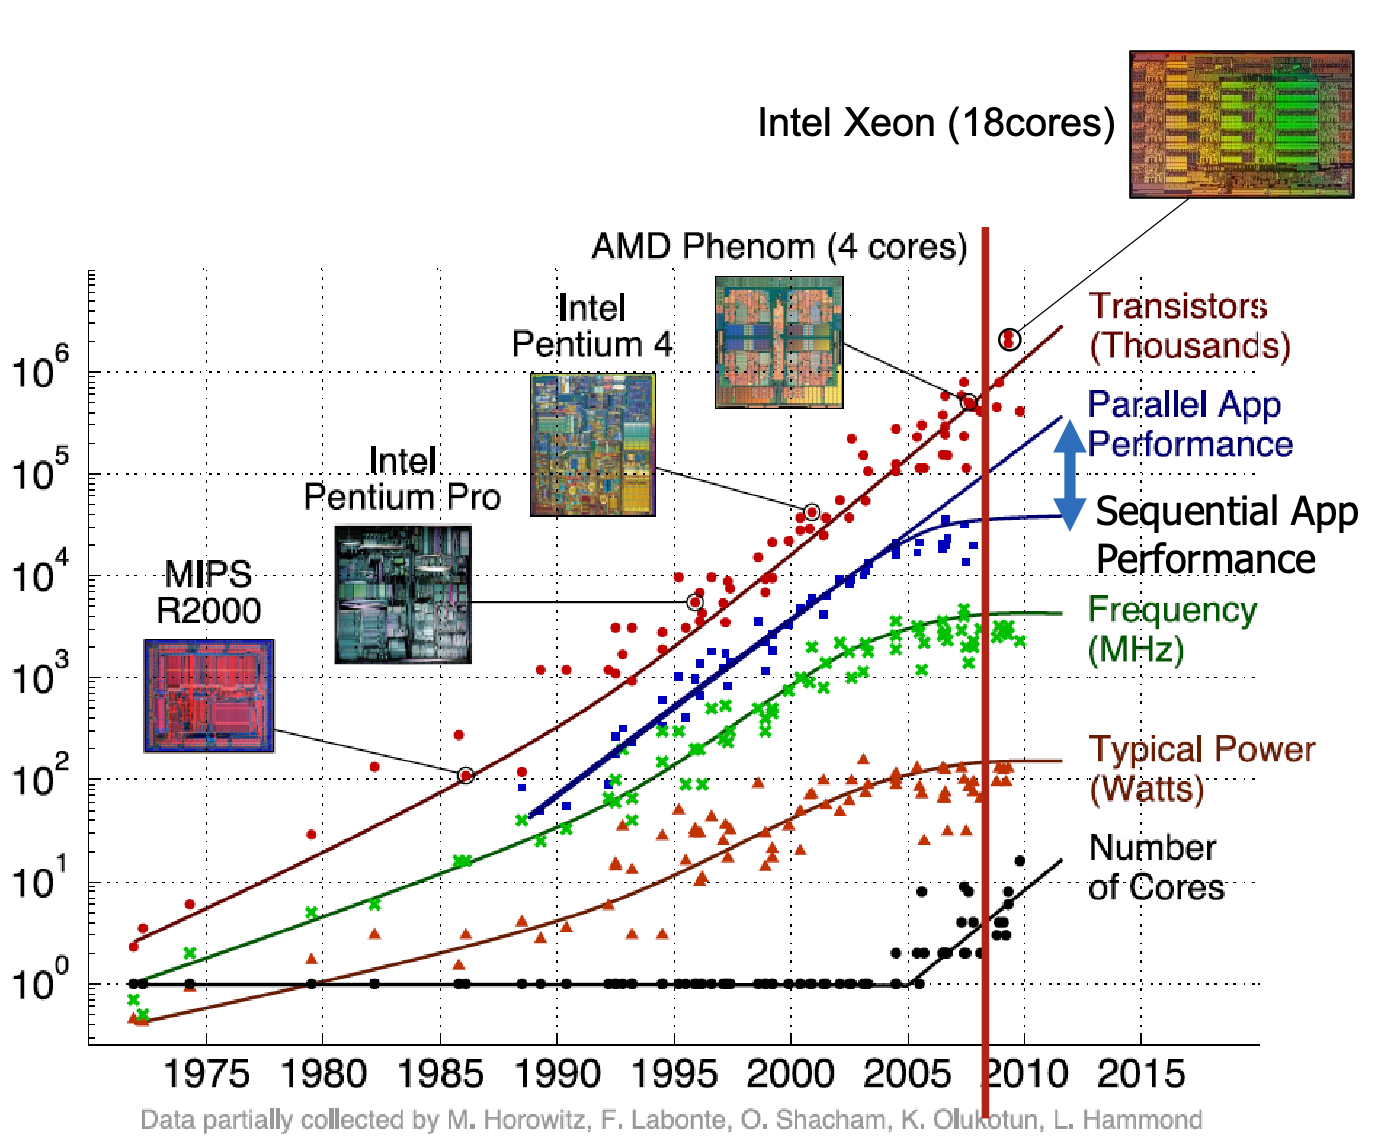
\includegraphics[width=.25\textwidth]{intro_1.png}
\end{wrapfigure}

\noindent$\sim$ 2005: plateau di consumo, frequenza e performance di programmi \textit{sequenziali}, aumento di performance di p.~che \textbf{sfruttano la parallelizzazione} $\rightarrow$ i programmi devono essere "consapevoli" che il processore \`e multicore!\\
Il compilatore mantiene un ruolo fondamentale: oltre a rendere meno "traumatico" il passaggio alla programmazione parallela, (non sono ancora auto-parallelizzanti) si interfaccia con i nuovi paradigmi di programmazione parallela offerti ai programmatori: il programmatore sfrutta interfacce semplici e astratte, mentre il compilatore traduce i costrutti in codice parallelo eseguibile (es. OpenMP)

\subsubsection{Eterogeneit\`a architetturale}

La programmazione parallela e il parallelismo architetturale sono oggi paradigmi consolidati, e i processori general purpose (seppur multicore e ottimizzati) non sono sufficienti per attivit\`a specializzate come la grafica $\rightarrow$ nascono componenti \textbf{acceleratori} di vario tipo: GPU, GPGPU, FPGA, TPU, NPU...
Questo complica ulteriormente la scrittura del software, e dunque impone altre evoluzioni nei compilatori e nelle ottimizzazioni.

\subsection{Ottimizzazione}

Ricordiamo le metriche usate:

\noindent\begin{minipage}[c]{.5\textwidth}
\begin{equation*}
  \text{Performance} = {{1}\over\text{Execution Time}}
\end{equation*}
\end{minipage}
\begin{minipage}[c]{.5\textwidth}
\begin{equation*}
  \text{Execution Time} = {\textcolor{blue}{\text{Instruction Count}} \times \textcolor{red}{\text{CPI}} \over \textcolor{red}{\text{Frequency}}}
\end{equation*}
\end{minipage}\\

Le ottimizzazioni possono avvenire dal punto di vista \textcolor{red}{HW (parametri architetturali)} e da quello \textcolor{blue}{SW (p.~di programma)}. Il compilatore pu\`o agire anche ad es. a livello di cache, aiutando a ridurre i miss e dunque i CPI delle istruzioni \lstinline|load| e \lstinline|store| (sappiamo che il costo di accesso aumenta di ordini di grandezza)

\subsubsection{Esempi di ottimizzazione}

\begin{emphasize}
  Distinguiamo le ottimizzazioni che avvengono a compile time o a runtime (statiche o dinamiche)
\end{emphasize}

\begin{itemize}
  \item \textbf{AS (Algebraic Semplification)}Semplification: ottimizzazione a runtime
  \begin{lstlisting}
-(-i); $\rightarrow$ i;
b or true; $\rightarrow$ true; //cortocircuito logico\end{lstlisting}
  \item \textbf{CF (Constant Folding)}:  valutare ed espandere espressioni costanti a compile time
  \begin{lstlisting}
c = 1+3; $\rightarrow$ c = 4;
(100<0) $\rightarrow$ false\end{lstlisting}
  
  \item \textbf{SR (Strength Reduction)}: sostituisco op. costose con altre pi\`u semplici: classico es. \lstinline|MUL| rimpiazzate da \lstinline|ADD/SHIFT| (esecuzione in 1 ciclo invece di multic.):\\
  \begin{minipage}[c]{.4\textwidth}
  \begin{lstlisting}
y = x*2;
y = x * 17;\end{lstlisting}
  \end{minipage}
  \hfill
  $\rightarrow$
  \hfill
  \begin{minipage}[c]{.4\textwidth}
  \begin{lstlisting}
y = x+x;
y = (x<<4) + x;\end{lstlisting}
  \end{minipage}\\
  es.~sofisticato: \lstinline|for| con operazioni su array, sostituito da operazioni su puntatori (aritmetica dei pt.) $\rightarrow$ il risultato si vede nel codice assembly\\
  \begin{minipage}[c]{.4\textwidth}
  \begin{lstlisting}
for (i=0; i<100; i++)
  a[i] = i*100;
  \end{lstlisting} 
  \end{minipage}
  \hfill
$\rightarrow$
  \hfill
  \begin{minipage}[c]{.4\textwidth}
  \begin{lstlisting}
t = 0;
for (; t<10000; t += 100) {
  *a = t;
  a = a + 4;
}\end{lstlisting}
  \end{minipage}
  
  \begin{minipage}[c]{.4\textwidth}
  \begin{lstlisting}
li s0, 0 // i = 0
li s1, 100
LOOP:
bge s0, s1, EXIT
slli s2, s0, 2
add s2, s2, a0
mul s3, s0, 100
sw s3, 0(s2)
addi s0, s0, 1
jal zero, LOOP
EXIT:\end{lstlisting} 
  \end{minipage}
  \hfill
$\rightarrow$
  \hfill
  \begin{minipage}[c]{.4\textwidth}
  \begin{lstlisting}
li s0, 0 // t = 0
li s1, 10000
LOOP:
bge s0, s1, EXIT
sw s0, 0(a0)
addi a0, a0, 4
jal zero, LOOP
EXIT:\end{lstlisting}
  \end{minipage}
  
\item \textbf{CSE (Common Subexpression Elimination)}: elimino i calcoli ridondanti di una stessa espressione riutilizzata in pi\`u istruzioni (statement)\\
  \begin{minipage}[c]{.4\textwidth}
    \begin{lstlisting}
y = b * c + 4
z = b * c - 1\end{lstlisting}
  \end{minipage}
\hfill $\rightarrow$ \hfill
\begin{minipage}[c]{.4\textwidth}
\begin{lstlisting}
x = b * c
y = x + 4
z = x - 1\end{lstlisting}
\end{minipage}
\item \textbf{DCE (Dead Code Elimination)}: elimino tutte le istruzioni che producono codice mai letto (e dunque utilizzato), es. variabili assegnate e mai lette, codice irraggiungibile $\rightarrow$ uno dei passi eseguiti pi\`u di frequente durante l'ottimizzazione del codice da parte del compilatore, per rimuovere anche tutto il dead code generato dagli altri passi di ottimizzazione\\
  \begin{minipage}[c]{.4\textwidth}
  \begin{lstlisting}
b = 3
c = 1 + 3
d = 3 + c\end{lstlisting}
  \end{minipage}
  \hfill $\rightarrow$ \hfill
  \begin{minipage}[c]{.4\textwidth}
  \begin{lstlisting}
c = 1 + 3
d = 3 + c\end{lstlisting}
  \end{minipage}

  \begin{minipage}[c]{.25\textwidth}
  \begin{lstlisting}
if (100<0)
{a = 5}\end{lstlisting}
  \end{minipage}
  \hfill $\rightarrow$ \hfill
  \begin{minipage}[c]{.25\textwidth}
  \begin{lstlisting}
if (false)
{}\end{lstlisting}
  \end{minipage}
  \hfill $\rightarrow$ \hfill
  \begin{minipage}[c]{.25\textwidth}
  \begin{lstlisting}

  \end{lstlisting}
  \end{minipage}
\item \textbf{Copy Propagation}: per uno statement \lstinline|x = y|, sostituisco gli usi futuri di \lstinline|x| con \lstinline|y| se non sono cambiati nel frattempo (propedeutico alla DCE)\\
  \begin{minipage}[c]{.25\textwidth}
  \begin{lstlisting}
x = y;
c = 1 + x;
d = y + c;\end{lstlisting}
  \end{minipage}
  \hfill $\rightarrow$ \hfill
  \begin{minipage}[c]{.25\textwidth}
  \begin{lstlisting}
x = y;
c = 1 + y;
d = y + c;\end{lstlisting}
  \end{minipage}
  \hfill $\tiny\underrightarrow{\text{DCE}}$ \hfill
  \begin{minipage}[c]{.25\textwidth}
  \begin{lstlisting}
c = 1 + y;
d = y + c;\end{lstlisting}
  \end{minipage}
\item \textbf{CP (Constant Propagation)}: sostituisco usi futuri di una variabile con assegnato valore costante con la costante stessa (se la variabile non cambia) (sempre ipotesi che i valori a fine es.~siano poi \textbf{usati}, e non dead code)\\
  \begin{minipage}[c]{.25\textwidth}
  \begin{lstlisting}
b = 3;
c = 1 + b;
d = b + c;\end{lstlisting}
  \end{minipage}
  \hfill $\tiny\underrightarrow{\text{CP}}$ \hfill
  \begin{minipage}[c]{.25\textwidth}
  \begin{lstlisting}
b = 3;
c = 1 + 3;
d = 3 + c;\end{lstlisting}
  \end{minipage}
  \hfill $\tiny\underrightarrow{\text{CF}}$ \hfill
  \begin{minipage}[c]{.25\textwidth}
  \begin{lstlisting}
b = 3;
c = 4;
d = 3 + c;\end{lstlisting}
  \end{minipage}
  \hfill $\tiny\underrightarrow{\text{CP}}$ \hfill

  \hfill $\tiny\underrightarrow{\text{CP}}$ \hfill
  \begin{minipage}[c]{.25\textwidth}
  \begin{lstlisting}
b = 3;
c = 4;
d = 3 + 4;\end{lstlisting}
  \end{minipage}
  \hfill $\tiny\underrightarrow{\text{CF}}$ \hfill
  \begin{minipage}[c]{.25\textwidth}
  \begin{lstlisting}
b = 3;
c = 4;
d = 7;\end{lstlisting}
  \end{minipage}
  \hfill $\tiny\underrightarrow{\text{DCE}}$ \hfill
  \begin{minipage}[c]{.25\textwidth}
  \begin{lstlisting}
d = 7;\end{lstlisting}
  \end{minipage}
\item LICM (Loop Invariant Code Motion): si occupa di muovere fuori dai loop tutto il codice \textbf{loop invariant}; evita i calcoli ridondanti\\
  \begin{minipage}[c]{.4\textwidth}
  \begin{lstlisting}
while (i < 100) {
  *p = x / y + i;
  i = i + 1;
}\end{lstlisting}
  \end{minipage}
  \hfill $\rightarrow$ \hfill
  \begin{minipage}[c]{.4\textwidth}
  \begin{lstlisting}
t = x / y;
while (i < 100) {
  *p = t + i;
  i = i + 1;
}\end{lstlisting}
  \end{minipage}
\end{itemize}

\subsubsection{Ottimizzazioni sui loop}

\begin{itemize}
  \item grande impatto sulla performance dell'intero programma (per ovvie ragioni)
  \item spesso sono ottimizzazioni propedeutiche a quelle machine-specific (effettuate nel backend): register allocation, instruction level parallelism, data parallelism, data-cache locality
\end{itemize}

\subsection{Anatomia di un compilatore}

\begin{figure}[h]
  \centering
  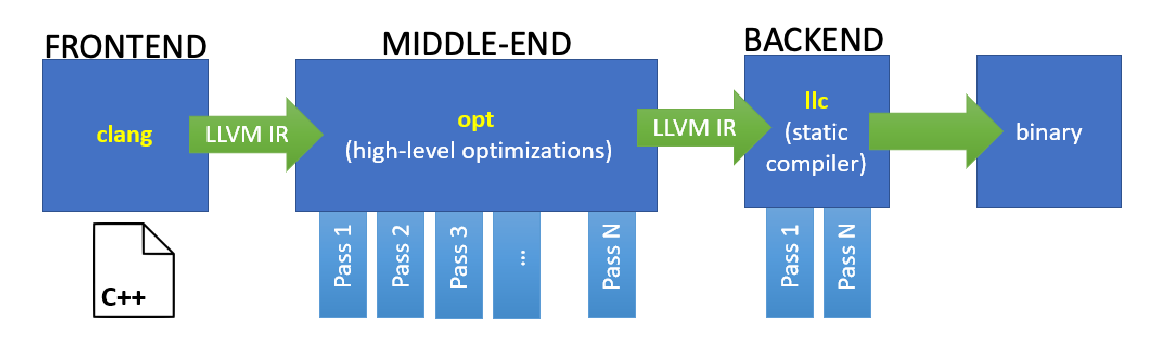
\includegraphics[width=.5\textwidth]{intro_3.png}
\end{figure}

\begin{itemize}
  \item almeno due compiti: \textbf{analisi del sorgente} e \textbf{sintesi di un programma in linguaggio macchina}, operando su una IR che si interpone tra frontend e backend, e tra source code e target code
  \item Il blocco di middle-end agisce su IR, e in vari passaggi lo trasforma e ottimizza ($\neq$ a seconda del compilatore)
  \item caso llvm: \lstinline|clang| (frontend) $\rightarrow$ \lstinline|opt| (middleend) $\rightarrow$ \lstinline|llc| (backend)
  \item \lstinline|opt| si basa su una serie di \textbf{passi di ottimizzazione (o di analisi)}: un passo di analisi scorre l'IR e lo analizza (non lo trasforma, ma produce informazioni utili); un passo di ottimizzazione sfrutta informazioni conosciute per trasformare l'IR (applica le ottimizzazione)
  \item alcune ottimizzazioni non possono essere effettuate o finalizzate senza conoscere l'architettura target (es. sulle cache), e dunque vengono eseguite dal backend
\end{itemize}

\subsubsection{Flag di ottimizzazione}

sono flag che passo al compilatore (al pass manager) per influenzare \textbf{ordine e numero dei passi di ottimizzazione}
\begin{multicols}{2}
\begin{itemize}
  \item \lstinline|-g|: solo debugging, nessuna ottimizzazione
  \item \lstinline|-O0|: nessuna ottimizzazione
  \item \lstinline|-O1|: solo ott. semplici
  \item \lstinline|-O2|: ott. pi\`u aggressive
  \item \lstinline|-O3|: ordine dei passi che sfrutta compromessi tra velocit\`a e spazio occupato
  \item \lstinline|-OS|: ottimizza per dimensione del compilato
\end{itemize}
\end{multicols}


\subsubsection{Uso di IR}

un backend che fa uso di IR permette di disaccoppiare con facilit\`a frontend e backend, lavorare su ottimizzazioni machine-independent, semplificare il supporto per molti linguaggi, eccetera

\begin{emphasize}
  Per supportare un nuovo linguaggio o una nuova architettura, basta scrivere un nuovo front/backend - il middle-end pu\`o rimanere lo stesso!
\end{emphasize}

\subsubsection{Ingredienti dell'ottimizzazione}

\begin{itemize}
  \item \textbf{formulare un problema di ottimizzazione} con molti casi di applicazione, sufficientemente efficiente e impattante su parti significative
  \item[$\rightarrow$] \textbf{rappresentazione} che astrae dettagli rilevanti $\rightarrow$ \textbf{analisi} di applicabilit\`a $\rightarrow$ \textbf{trasformazione del codice} $\rightarrow$ \textbf{testing} $\rightarrow \, \circlearrowleft$
\end{itemize}

\vspace{-2em}
\section{Rappresentazione intermedia}

Ricordiamo: middle end come sequenza di passi, di analisi o di trasformazione $\rightarrow$ per analizzare e trasformare il codice occorre una rappr.~intermedia (IR) \textbf{espressiva} che \textbf{mantenga le informazioni importanti da un passo all'altro}

\vspace{-1em}
\subsection{Propriet\`a di una IR}

scegliamo IR diverse a seconda del loro uso, in generale alcune caratteristiche sono sempre richieste:
\begin{itemize}
  \item facilit\`a di \textbf{generazione} (effetti sul frontend)
  \item facilit\`a e costo di \textbf{manipolazione}
  \item livello di astrazione e di \textbf{dettaglio esposto}: effetti su frontend e backend ($\neq$ IR da un lato e dall'altro, a seconda di astraz.~e dettaglio necessari)
\end{itemize}

\vspace{-1em}
\subsection{Tipi di IR}

\begin{itemize}
  \item AST (abstract syntax tree)
  \item DAG (grafi diretti aciclici)
  \item 3AC (3-address code): simile all'assembly (3 indirizzi: registro destinazione e max 2 operandi)
  \item SSA (Static Single Assignment): evoluzione di 3ac con ulteriori propriet\`a di control flow
  \item CFG (control flow graphs): rappresenta "come" vengono chiamate le funzioni (a partire dal main)
  \item CG (call graph)
  \item PDG (program dependence graphs): fondamentale per lavorare sul parallelismo, multithreading...
\end{itemize}

\vspace{-1em}
\begin{emphasize}
  Le ott.~inter-procedurali devono per forza basarsi su IR di tipo CG (es. per decidere quando fare \textbf{inlining} - espandere il codice della funzione invece di chiamarla - evidente tradeoff tra dimensione del codice e overhead dovuto alla chiamata di funzione)
\end{emphasize}

\subsection{Categorie di IR}

\begin{itemize}
  \item grafiche (o strutturali)
    \begin{itemize}
      \item orientate ai grafi
      \item molto usate nella source-to-source translation, tipicam.~per ott.~che non hanno bisogno della struttura sofisticata di un middle-end\\
      es.~openMP: di fatto annotazioni sul codice, come strumento semplice per la parall.~(es. \textbf{outlining}: prendo es un loop e lo impacchetto in una funzione che poi dovra essere eseguita dai thread per la parallelizzazione) - non sto ottimizzando nel senso proprio del termine, ma sto trasformando il codice e lo sto rendendo eseguibile in maniera parallela
      \item solitamente voluminose (basate su grafi) - tradeoff con il fatto che non coinvolgono il middle-end
      \item es.~AST, DAG
    \end{itemize}
  \item lineari
    \begin{itemize}
      \item pseudocodice per macchine astratte
      \item livello di astrazione vario
      \item strutture dati semplici e compatte
      \item facile da riarrangiare (evidentemente il pi\`u comodo per eseguire le ottimizzazioni)
      \item es. 3AC
    \end{itemize}
  \item ibride (sfruttano combinazioni delle prime due) (es.~CFG)
\end{itemize}
\subsection{Esempi di rappresentazione}


\subsubsection{Sintassi concreta (testo)}

Pi\`u semplice in quanto pi\`u vicina al livello di astrazione "umano" di ragionamento sul programma, ma non il livello corretto per ottimizzare ne comprendere correttamente la semantica del programma

\begin{lstlisting}[language=java]
let value = 8;
let result = 1;
for (let i = value; i>0; i = i - 1) {
  result = result * i;
}
console.log(result);\end{lstlisting}

\vspace{-.5em}
\subsubsection{AST (Abstract Syntax Tree)}

Albero i cui nodi rappresentano diverse parti del programma: il nodo radice rappresenta il \textbf{programma}, il quale a sua volta contiene un blocco di istruzioni dal quale discendono tanti figli quante le sue istruzioni

\vspace{1em}
\noindent\begin{minipage}[c]{.3\textwidth}
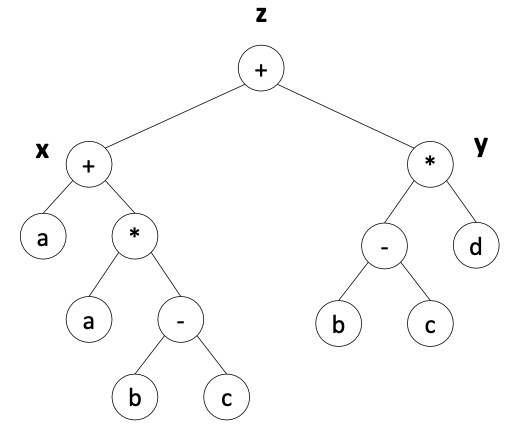
\includegraphics[width=\textwidth]{ir_1.png}
\end{minipage}\hfill
\begin{minipage}[c]{.67\textwidth}
\begin{lstlisting}[linewidth=.5\linewidth]
x = a + a * (b - c)
y = (b - c ) * d
z = x + y\end{lstlisting}
\textbf{PRO}: molto comodo per interpreti (basta usare una fz.~ricorsiva per processare l'albero)

\textbf{CONTRO}: un nodo \`e un oggetto troppo generico $\rightarrow$ analizzare un ast per l'ottimizzazione impone ogni volta di ragionare sulla differenza semantica tra i nodi (complica molto)
\end{minipage}


\vspace{-.5em}
\subsubsection{DAG (Directed Acyclic Graph)}

Contrazione di ast che evita la duplicazione di espressioni $\rightarrow$ \textbf{rappresentazione pi\`u compatta}

\noindent\textbf{Limite}: il riuso e possibile solamente dimostrando che il suo \textbf{valore non cambia} nel programma
\begin{emphasize}
  essendo assegnamenti e chiamate frequentissimi, il fatto che il dag non abbia nozione di come le espr.~cambino valore nel tempo non lo rende un buon candidato per le ottimizzazioni
\end{emphasize}

\begin{example}[frametitle={Esempi}]
   \noindent\begin{minipage}[c]{.18\textwidth}
   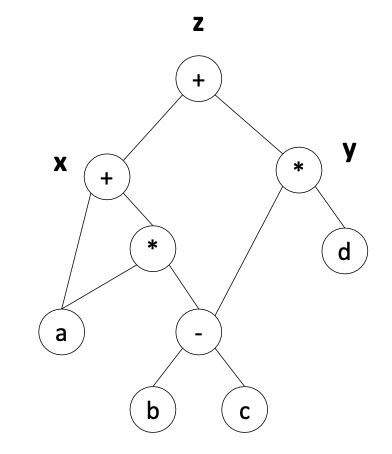
\includegraphics[width=\textwidth]{ir_2.png}
   \end{minipage}
   \begin{minipage}[c]{.23\textwidth}
      \begin{lstlisting}
x = a+a*(b-c);
y = (b-c)*d;
z = x+y;
# espr. trovate
t1 = b-c;
t2 = a*t1;
x = a+t2;
y = t1*d;
z = x+y;\end{lstlisting}
   \end{minipage}\hfill\vline\hfill
   \begin{minipage}[c]{.18\textwidth}
   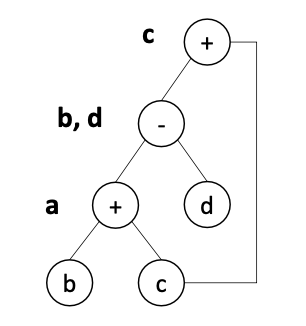
\includegraphics[width=\textwidth]{ir_3.png}
   \end{minipage}
   \begin{minipage}[c]{.35\textwidth}
      \begin{lstlisting}
a = b + c;
b = a - d;
c = b + c;
d = a - d;
# espr. trovate (ERRORE)
a = b + c; # cambia val.
d = a - d;
c = d + c;\end{lstlisting}
   \end{minipage}
\end{example}



\subsubsection{3AC (3-Address Code)}

\begin{minipage}[c]{.65\textwidth}
Evidentemente adatto: tutte le istr.~del programma vengono spezzettate in istr.~di forma semplice simile all'assembly, di tipo \lstinline|x = y op z| (1 operatore, massimo 3 operandi)

\noindent\hfill
  \begin{minipage}[c]{.3\textwidth}
    \begin{lstlisting}
x - 2 * y\end{lstlisting}
  \end{minipage}\hfill
  $\rightarrow$\hfill
  \begin{minipage}[c]{.32\textwidth}
    \begin{lstlisting}
t1 = 2 * y
t2 = x - t1\end{lstlisting}
  \end{minipage}\hfill
\end{minipage}
  \hfill
  \begin{minipage}[c]{.3\textwidth}
  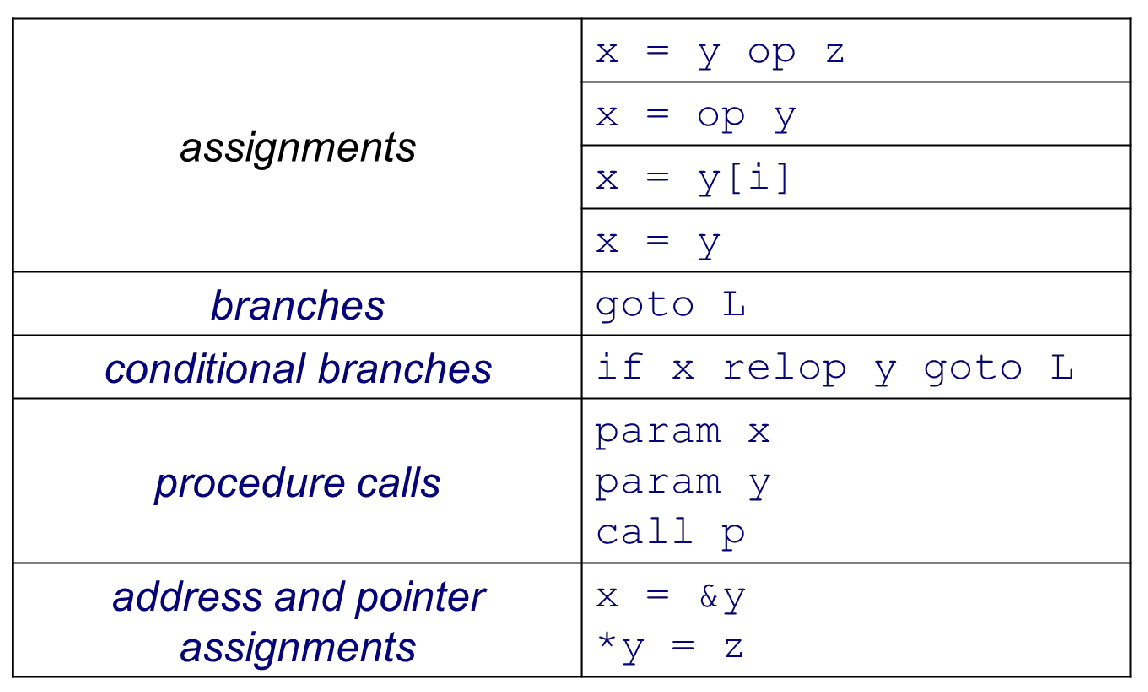
\includegraphics[width=\textwidth]{ir_4.png}
  \end{minipage}

\textbf{PRO}:
\begin{itemize}
  \item espressioni complesse spezzettate
  \item forma compatta e simil-assembly
  \item registri temporanei \textbf{intermedi, virtuali e illimitati} (tralascio problemi architetturali - n.~di r.~fisici a disposizione e eventuali op. di spill, cio\`e aggiungere load o store in mancanza di r.~fisici)
\end{itemize}

\paragraph{Varianti di 3AC}~\\

A seconda dei vincoli che ho per l'implementazione pratica:\\

\noindent\begin{minipage}[c]{.7\textwidth}
\begin{itemize}
  \item \textbf{quadruple}: id istruzione, opcode, i 3 registri $\rightarrow$ semplice struttura record, facile da analizzare e riordinare ma i nomi espliciti prendono pi\`u spazio
  \item \textbf{triple}: id istruzione, opcode, 2 operandi $\rightarrow$ uso l'indice dell'espressione nell'array come "nome" del registro destinazione $\rightarrow$ risparmio spazio, ma diventa piu complesso da analizzare (nomi impliciti) e riordinare
\end{itemize}
\begin{emphasize}[frametitle={Inapplicabilit\`a diretta della Constant Propagation con forma 3AC}]
  La CP \`e applicabile solo se la variabile \textbf{se non cambia nel frattempo} $\rightarrow$ una IR di tipo 3AC non pu\`o applicarla immediatamente (devo prima analizzare il resto del codice)
\end{emphasize}
\end{minipage}
\begin{minipage}[c]{.3\textwidth}
\centering
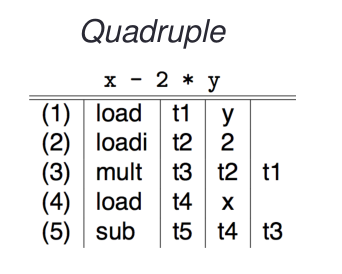
\includegraphics[width=.7\textwidth]{ir_5.png}
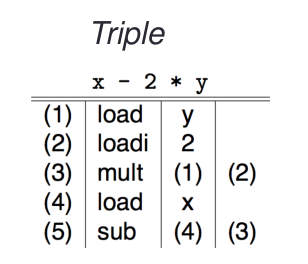
\includegraphics[width=.7\textwidth]{ir_6.png}
\end{minipage}

\subsubsection{SSA (Static Single Assignment)}

\begin{itemize}
  \item Evoluzione di 3AC che impone che la \textbf{definizione (assegnamento)} delle variabili avvenga \textbf{solo una volta} (def.~multiple sono tradotte in multiple versioni della var)
  \item \textbf{PRO}: ogni definizione ha associata direttamente una \textbf{lista di tutti i suoi usi} - semplifica enormemente le ottimizzazioni di tipo CP e non solo
\end{itemize}


\begin{emphasize}
  Quasi sempre uno dei passi di ottimizzazione prevede il passaggio a forma SSA
\end{emphasize}

\begin{emphasize}
  La scelta della IR dipende ovviamente dal livello di dettaglio necessario per ogni specifico compito $\rightarrow$ \textbf{in un compilatore coesistono pi\`u IR} (anche per questo esistono forme ibride)
\end{emphasize}

\subsubsection{CFG (Control Flow Graph)}

\noindent\begin{minipage}[c]{.65\textwidth}
\begin{itemize}
  \item modella il trasferimento (flusso) del controllo in un programma tra \textbf{blocchi} di istruzioni
  \item permette di aggiungere informazioni sui \textbf{salti} al di sopra di una IR lineare
  \item i suoi nodi sono Basic Block
  \item gli archi rappresentano il flusso di controllo del programma (loop, condizioni, ecc.)
\end{itemize}
\end{minipage}
\begin{minipage}[c]{.35\textwidth}
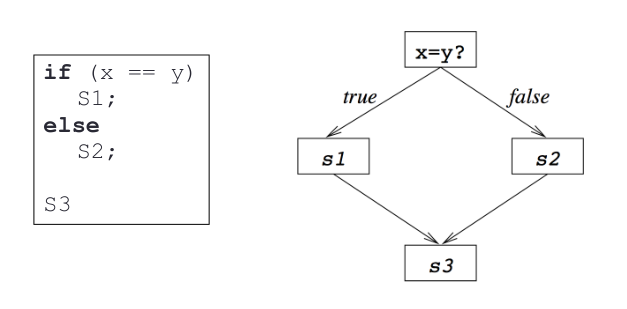
\includegraphics[width=\textwidth]{ir_7.png}
\end{minipage}

{%
  \begin{wrapfigure}{r}{.325\textwidth}
		\vspace{5em}
    \hfill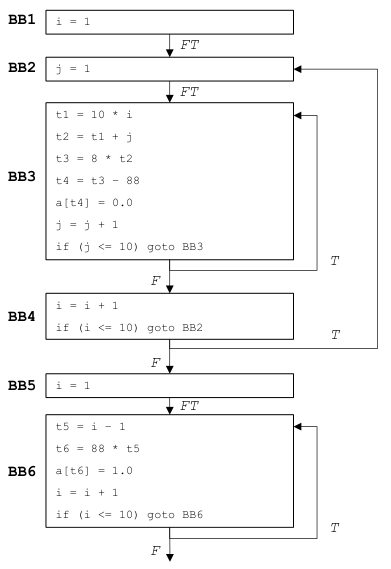
\includegraphics[width=0.3\textwidth]{ir_8.png}
		\captionof{figure}{Esempio di CFG}
  \end{wrapfigure}
	\noindent\par \begin{itemize}
		\item un BB \`e una seq.~di istruzioni in forma 3AC
			\begin{itemize}
				\item singolo \textit{entry point}: solo la prima istruzione puo essere raggiunta dall'esterno
				\item singolo \textit{exit point}: se eseguo la prima istr.~\textbf{devo eseguire tutte le altre} - garantisco che venga \textbf{eseguito interamente}
				\item Le chiamiamo sezioni single-entry, single-exit (possono essere sezioni anche piu grandi, ma le piu piccole di questo tipo sono i BB)
			\end{itemize}
		\item un arco connette due nodi $B_{i}\rightarrow B_{j}$ $\iff$ $b_{j}$ pu\`o eseguire dopo $B_{i}$ in qualche percorso del ctrl flow del programma
			\begin{itemize}
				\item prima istr.~di $B_{j}$ \`e target dell'istr.~di salto al termine di $B_{i}$
				\item[$\lor$] $B_{i}$ non ha un istr.~di salto come ultima istr.~(nodo \textit{falltrough}) e $B_{j}$ \`e suo unico successore
			\end{itemize}
		\item un CFG \textbf{normalizzato} ha i BB \textbf{massimali}
			\begin{itemize}
				\item non possono essere resi pi\`u grandi senza violare condizioni
				\item unisco i BB fallthrough che non hanno label all'inizio
				\item posso avere CFG non norm.~dopo qualche generico passo di ottimizzazione (non le facciamo accadere "spontaneamente")
			\end{itemize}
	\end{itemize}%
}


\paragraph{Algoritmo per la costruzione del CFG}~\\

\begin{enumerate}
  \item identificare il \textbf{leader} di ogni BB:
    \begin{itemize}
      \item la prima istruzione
      \item il target di un salto
      \item ogni istruzione dopo un salto
    \end{itemize}
  \item il BB \textbf{comincia} con il leader e \textbf{termina} con l'istruzione immediatamente precedente un nuovo leader (o l'ultima istruzione)
  \item \textbf{connettere} i BB tramite archi di 3 tipi:
    \begin{itemize}
      \item \textbf{fallthrough} (o fallthru): esiste solo un percorso che collega i due blocchi
      \item \textbf{true}: il secondo blocco \`e raggiungibile dal primo se un condizionale \`e \lstinline|true|
      \item \textbf{false}: il secondo blocco \`e raggiungibile dal primo se un condizionale \`e \lstinline|false|
    \end{itemize}
\end{enumerate}

\subsubsection{DG (Dependency Graph)}

I nodi di un DG sono istruzioni; un arco connette due nodi di cui \textbf{uno usa il valore definito dall'altro}. Sono indispensabili per l'\textit{instruction scheduling} e per mantenere il CPI della pipeline (ricordiamo quella RISC-V):\\

\noindent\begin{minipage}[c]{.6\textwidth}
\begin{itemize}
  \item[$\curvearrowright$] IF Instruction Fetch
  \item[$\downarrow$] ID Instruction Decode
  \item[$\downarrow$] EXE Execute
  \item[$\downarrow$] MEM Memory Access
  \item[$\hookleftarrow$] WB Write Back
\end{itemize}
\end{minipage}
\begin{minipage}[c]{.4\textwidth}
  \centering
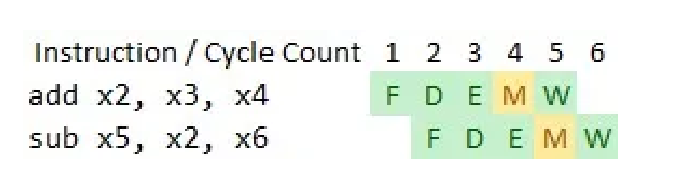
\includegraphics[width=.85\textwidth]{ir_9.png}
\captionof{figure}{Esempio di data hazard}
\end{minipage}\\

\begin{example}[frametitle={Esempio: risultato di una \lstinline|add|}]
   Se in fase di decode provo a leggere il registro usato in una \lstinline|add| immediatamente precedente, questo ancora non contiene il risultato aggiornato (pronto appena tra 2 cicli) $\rightarrow$ \textbf{data hazard}, gestito solitamente dalla \textbf{forwarding unit} che bypassa MEM e WB e inoltra direttamente il dato 
\end{example}

\begin{emphasize}[frametitle={Soluzione generica (inefficiente)}]
  Per quanto i controlli vengano svolti dalla fw.~unit, in generale l'unico modo per evitare questo tipo di hazard \`e distanziare le istruzioni tra loro affinch\'e il dato sia disponibile $\rightarrow$ inserisco nop (cicli di stallo), ma vado a "rompere" l'IPC pari a a 1 della pipeline sempre piena ($<$ performance)
  \mdfsubtitle{Soluzione migliore}
  \textbf{scheduling} del programma, spostando istruzioni che non dipendono da quei registri al posto di aggiungere \lstinline|nop| $\rightarrow$ uno dei compiti principali di un backend, che per evitare di cercare le istruzioni libere "manualmente" sfrutta la IR di tipo DG che fornisce esattamente le informazioni sulle dipendenze tra istruzioni
\end{emphasize}

\subsubsection{DDG (Data Dependency Graph)}

\begin{itemize}
  \item specifico per multicore e parallelismo, usato per dare una rappresentazione tra le dipendenze dei \textbf{dati} - tipicamente i loop, a patto che non ci siano dipendenze di dato tra le varie iterazioni.
  \item tipicamente uso il \textbf{polyhedral model} $\rightarrow$ rappresento lo spazio delle it.~come un poliedro (a seconda del numero di loop innestati), che permette di capire se esiste qualche permutazione dei loop (direzione di attraversamento dello spazio delle iterazioni; ovvero ad esempio scambiare l'ordine dei loop) \textbf{non soggetta a dipendenze}
\end{itemize}

\subsubsection{CG (Call Graph)}

\noindent\begin{minipage}[c]{.6\textwidth}
Rappresentazione gerarchica a grafo usata per ragionare sull'insieme delle potenziali chiamate tra funzioni della translation unit del sorgente

\begin{emphasize}[frametitle={Nota}]
  Il compilatore ha visibilit\`a solo fino a livello dei singoli moduli: posso estendere le ottimizzazioni al massimo fino ai legami tra funzioni dello stesso modulo, quelle pi\`u ampie si spostano a framework di ott.~che agiscono es.~a livello di linker
\end{emphasize}
\end{minipage}
\begin{minipage}[c]{.4\textwidth}
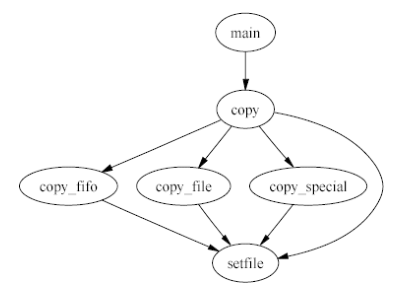
\includegraphics[width=\textwidth]{ir_10.png}
\end{minipage}

\section{Ottimizzazione locale e Local Value Numbering}

\subsection{Scope dell'ottimizzazione}

\noindent\begin{minipage}[c]{.55\textwidth}
Lo scope viene influenzato da come viene gestito il flusso di controllo in un programma

\begin{itemize}
  \item ott.~\textbf{\textcolor{Emerald}{locale}}: entro un singolo BB, non si preoccupa del flusso
  \item ott.~\textbf{\textcolor{Orange}{globale}}: lavora a livello dell'intero CFG
  \item ott.~\textbf{\textcolor{Cerulean}{interprocedurale}}: lavora a livello del call graph, e quindi sui CFG di pi\`u funzioni
\end{itemize}
\end{minipage}\hfill
\begin{minipage}[c]{.4\textwidth}
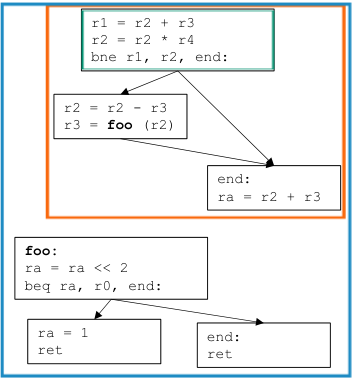
\includegraphics[width=\textwidth]{lvn_1.png}
\end{minipage}

\subsection{Dead Code Elimination}

Cominciamo ragionando su ott.~locali come la DCE (sono \textit{dead code} le istr.~che definiscono una variabile mai utilizzata)

\noindent\begin{minipage}[b]{.65\textwidth}
Sicuramente va tolta la def.~di c, ma poich\'e \lstinline|print| \textbf{non definisce nulla}, stando alla def.~\`e dead code! $\rightarrow$ Estendiamo la definizione dicendo che lo sono le istr \textbf{prive di side effects} che definiscono ... 
\end{minipage}\hfill
\begin{minipage}[c]{.3\textwidth}
\begin{lstlisting}
main {
  int a = 4;
  int b = 2;
  int c = 1;
  int d = a + b;
  print d;
}\end{lstlisting}
\end{minipage}

\subsubsection{Algoritmo per la DCE}

\begin{enumerate}
  \item $\forall$ istruzione in BB
    \begin{itemize}
      \item aggiungi operandi ad un metadato array \lstinline|used|
    \end{itemize}
  \item $\forall$ istruzione in BB
    \begin{itemize}
      \item se non ha destinazione e non ha side effects rimuovila
      \item altrimenti se la destinazione non corrisponde a nessuno degli elem di \lstinline|used| rimuovila
    \end{itemize} 
\end{enumerate}

\begin{lstlisting}
used = {};

for instr in BB:
  used += instr.args;

for instr in BB:
  if instr.dest &&
     instr.dest not in used:
        delete instr\end{lstlisting}

A questo punto rendiamolo iterativo, per farlo eseguire fino a "convergenza" (elimino tutto il \textit{d-c})
  
\begin{lstlisting}
while prog changed:
{
  ... #alg
}\end{lstlisting}

\noindent\begin{minipage}[c]{.3\textwidth}
\begin{lstlisting}
main {
	int a = 100;
	int a = 42;
	print a;
}\end{lstlisting}
\end{minipage}\hfill $\rightarrow$ \hfill
\begin{minipage}[c]{.62\textwidth}
Consideriamo questo esempio in cui si ridefinisce una variabile: il nostro algoritmo corrente non elimina nulla perch\'e non gestisce le \textbf{dead stores}
\end{minipage}

\noindent $\rightarrow$ per estenderlo dobbiamo poter \textbf{rilevare gli assegnamenti multipli} di una variabile, e quindi anche \textbf{preoccuparci dell'ordine} delle istruzioni! (pi\`u complicato senza forma SSA)

\begin{itemize}
  \item dopo ogni istr.~teniamo traccia delle variabili definite, ma non usate
  \item se troviamo un altro assegnamento alla stessa variabile prima della fine del blocco sappiamo che quello precedente pu\`o essere eliminato
\end{itemize}

\begin{lstlisting}
last_def = {}; /* lista di variabili definite ma non usate (ptr alla piu' recente per le sole variabili mai usate) */

for instr in BB:
	last_def -= instr.args; /*rimuovo ogni argomento (operando) dell'istruzione corrente: se presente, e' un uso della variabile */

	if instr.dest in last_def:
		delete last_def[instr.dest]; /*se a questo punto la destinazione dell'istr. corrente e' presente in last_def posso sovrascrivere la definizione precedente*/
	last_def[instr.dest]=instr;\end{lstlisting}

\begin{itemize}
  \item nota: per situazioni tipo \lstinline|x=2; x=x+3;| si vuole evitare che la seconda istr.~venga eliminata perch\'e non ho realizzato che \lstinline|x| \`e usata (non \`e \textit{d-c}) $\rightarrow$ per questo controllo prima gli usi e poi le definizioni
  \item anche questo algoritmo va ripetuto fino a convergenza
\end{itemize}


\subsection{Local Value numbering}

Tecnica utilizzata per considerare il concetto di ordine delle definizioni in assenza di propriet\`a di tipo SSA

osserviamo 3 pattern che forniscono opportunit\`a di eliminazione di codice ridondante:
\begin{itemize}
  \item dead code elimination: 1 variabile e piu valori
  \item copy propagation: 1 valore e piu variabili
  \item common subexpression elimination: 1 valore (in forma di espressione) e piu variabili
\end{itemize}

sono tutti modelli di computazione che si focalizzano sulle \textbf{variabili} $\rightarrow$ focalizzandoci sui \textbf{valori} possiamo eliminare tutte le forme di ridondanza

\begin{figure}[h]
  \centering
  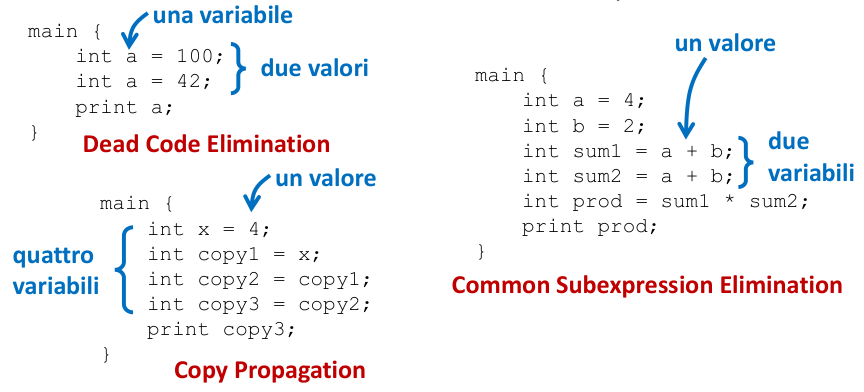
\includegraphics[width=.65\textwidth]{lvn_2.png}
  \caption{Esempi di codice legati ai pattern citati}
\end{figure}

\begin{itemize}
	\item costruisco un metadato in forma di tabella che riscrive le espr.~(istruzioni) in funzione dei valori gia osservati $\rightarrow$ evitando di riassegnare lo stesso valore a piu variabili si evita la ridondanza
	\item analizzo le istruzioni in termini del value, e in caso questo coincida con entry della tabella gi\`a presenti punto direttamente a quella
\end{itemize}

\begin{example}
	\noindent\begin{minipage}[c]{.6\textwidth}
		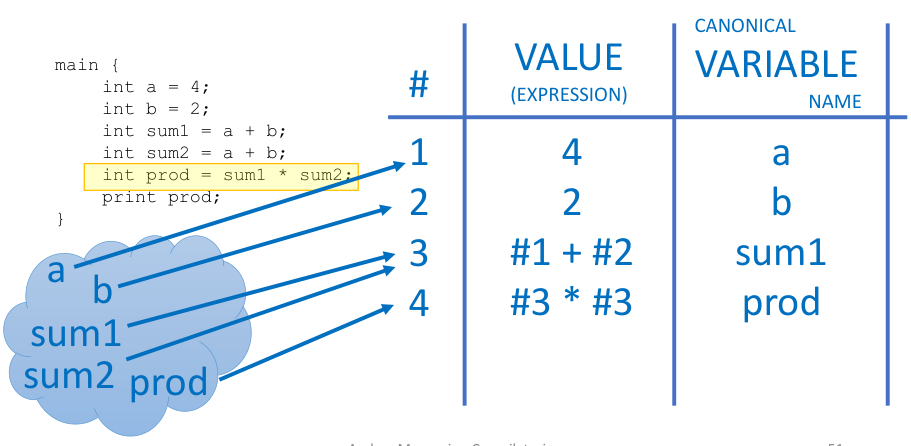
\includegraphics[width=\textwidth]{lvn_3.png}
		\captionof{figure}{Esempio di ottimizzazione tramite LVN}
	\end{minipage}\hfill
	\begin{minipage}[c]{.3\textwidth}
		\centering
		\begin{lstlisting}
	main {
		int a = 4;
		int b = 2;
		int sum1 = a + b;
		int prod = sum1 * sum1;
		print prod;
	}\end{lstlisting}

	Risultato ottenuto
\end{minipage}
\end{example}


\noindent\begin{minipage}[c]{.3\textwidth}
\begin{lstlisting}
#...
int sum1 = a + b;
int sum2 = b + a;\end{lstlisting}
\end{minipage}\hfill $\rightarrow$
\begin{minipage}[c]{.65\textwidth}
Semplice variante del programma non riconosciuta dall'algoritmo (non conosce la pr.~commutativa della somma) $\rightarrow$ vado a \textbf{canonicalizzare} l'algoritmo, ovvero imporre un ordine numerico tra le entry (i valori) e usarle sempre in ordine crescente per le op.~commutative (di fatto svolto da tutti i compilatori)
\end{minipage}

\section{Data Flow Analysis}

\subsection{Cos'\`e la DFA}

La possiamo vedere come una \textbf{metodologia} o come un \textbf{framework} di analisi, applicabile a vari problemi di ottimizzazione (CP, CSE, DCE, ...)

\begin{itemize}
  \item analisi \textbf{locale}: si focalizza sull'effetto di ogni istruzione $\rightarrow$ posso comporre gli effetti di tutte le istr.~per derivare informazione dall'inizio del BB ad ogni istruzione
  \item analisi \textbf{globale} (DFA): simile, ma molto pi\`u complessa $\rightarrow$ analizza l'effetto di ogni BB, e poi ha una metodologia per comporre l'effetto dei BB ai \textbf{confini} degli stessi per derivare informazione
\end{itemize}

La DFA \`e \textbf{sensibile al flusso di controllo in una funzione} e prevede un'analisi \textbf{intraprocedurale} (singola funzione, singolo CFG)

\begin{example}
	\noindent\begin{minipage}[c]{.3\textwidth}
		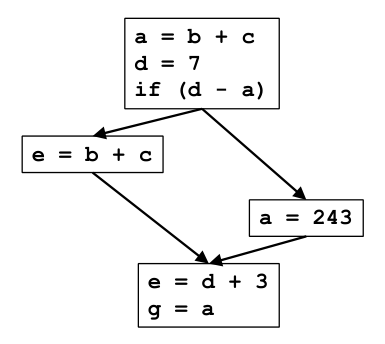
\includegraphics[width=\textwidth]{dfa_1.png}
	\end{minipage}\hfill
	\begin{minipage}[c]{.65\textwidth}
		La DFA ci permette di derivare informazioni da un CFG, ad esempio $\forall$ variabile \lstinline|x| in ogni punto del grafo:
		\begin{itemize}
			\item qual \`e il suo valore?
			\item quale "definizione" la definisce?
			\item la definizione \`e ancora "valida" (\textit{live})?
		\end{itemize}
	\end{minipage}

\begin{emphasize}
	Queste risposte normalmente le otteniamo grazie alla forma SSA delle istruzioni e alla struttura di LLVM, ma qui stiamo ancora "costruendo" la forma SSA
\end{emphasize}
\end{example}

\subsubsection{Rappresentazione del programma statica o dinamica}

\begin{itemize}
	\item \textbf{statica}: programma finito, un pezzo di codice $\rightarrow$ molto facile da analizzare
	\item \textbf{dinamica}: pu\`o avere infiniti percorsi di esecuzione, rappresenta una possibile esecuzione reale!
		\begin{itemize}
			\item es. loop che si basa sull'analisi di un input
		\end{itemize}
		\begin{emphasize}
			condizioni che un compilatore \textbf{non pu\`o analizzare}, soprattutto non in maniera statica e \textit{finita} in termini di possibili istanze $\rightarrow$ spesso si passano al comp.~informazioni di "profiling" misurate durante ripetute esecuzioni del programma pre-ottimizzato
		\end{emphasize}
\end{itemize}

\noindent $\rightarrow$ Con la DFA siamo in grado di dire qualcosa \textbf{per ogni punto del programma}, combinando informazioni relative a \textbf{tutte le possibili istanze} dello stesso p.to

\subsubsection{Effetti di istruzioni e BB}

Effetti di un'istruzione: (\lstinline|a = b + c;|)
\begin{itemize}
  \item \textbf{uses}: delle variabili (\lstinline|b,c|)
  \item \textbf{kills}: una precedente definizione (\lstinline|a|)
  \item \textbf{defines}: una variabile (\lstinline|a|)
\end{itemize}
Combinando gli effetti delle singole istr.~si definiscono gli \textbf{effetti di un BB}:
\begin{itemize}
  \item \textbf{uso localmente esposto} (\textit{locally exposed use}): in un BB \`e un uso di una var.~che non \`e preceduto nel BB da una definizione della stessa variabile
  \item ogni definizione di una var.~nel BB \textbf{killa} tutte le definizioni delal stessa variabile che \textbf{raggiungono} il BB
  \item \textbf{definizione localmente disponibile} (\textit{locally available definition}): ultima definizione di una variabile nel BB
\end{itemize}

\newpage
\begin{example}
\noindent \begin{minipage}[c]{.45\textwidth}
    \begin{lstlisting}[numbers=right,numbersep=-10pt]
t1 = r1+r2
r2 = t1
t2 = r2+r1
r1 = t2
t3 = r1*r1
r2 = t3
if r2>100 goto L1\end{lstlisting}
\end{minipage}\hfill
\begin{minipage}[c]{.55\textwidth}
\begin{itemize}
  \item usi loc.~esposti: 1 (\lstinline|r1,r2|), 3 (\lstinline|r2|), ...
  \item kill: 2 (\lstinline|r2|), ...
  \item definizioni loc.~disponibili: 6 (\lstinline|r2|), 5 (\lstinline|t3|), ...
\end{itemize}
\end{minipage}
\end{example}

\subsection{Reaching Definitions}

\noindent \begin{minipage}[c]{.6\textwidth}
Primo esempio di problema inquadrabile e risolvibile mediante DFA
\begin{itemize}
  \item ogni istruzione di assegnamento \`e una definizione
  \item una definizione \textit{d} raggiunge (reaches) un punto it\textit{p} se esiste un percorso da \textit{d} a \textit{p} tale per chu d non \`e uccisa (sovrascritta) lungo quel percorso
\end{itemize}
\end{minipage}
\hfill
\begin{minipage}[c]{.3\textwidth}
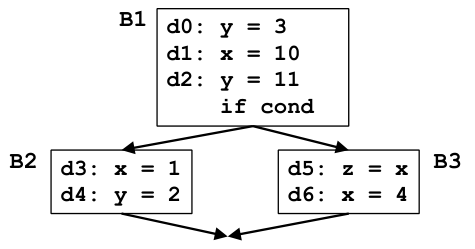
\includegraphics[width=\textwidth]{dfa_2.png}
\captionof{figure}{Esempio}
\end{minipage}

Definizione del problema:
\begin{itemize}
  \item determinare \textbf{per ogni punto} del programma se \textbf{ogni definizione} nel programma \textbf{raggiunge} quel punto
  \item[$\rightarrow$] usiamo un \textbf{bit vector} per ogni istruzione, con lunghezza del vettore pari al numero di definizioni $\Rightarrow$ diventa una sorta di matrice con righe le istruzioni, colonne le definizioni
\end{itemize}

\begin{example}
      \centering
      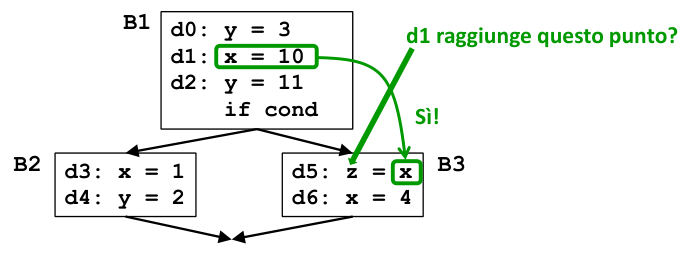
\includegraphics[width=.45\textwidth]{dfa_3.png}\hfill
      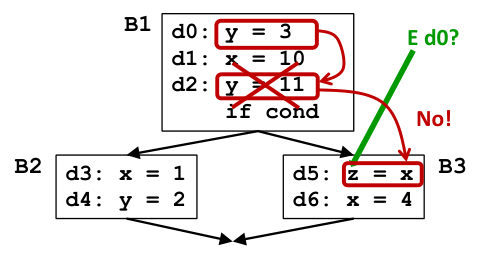
\includegraphics[width=.35\textwidth]{dfa_4.png}\\
      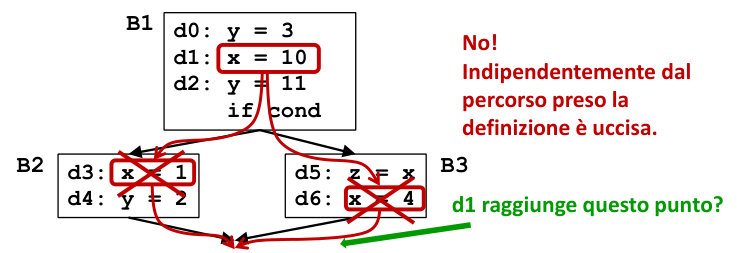
\includegraphics[width=.45\textwidth]{dfa_5.png}\hfill
      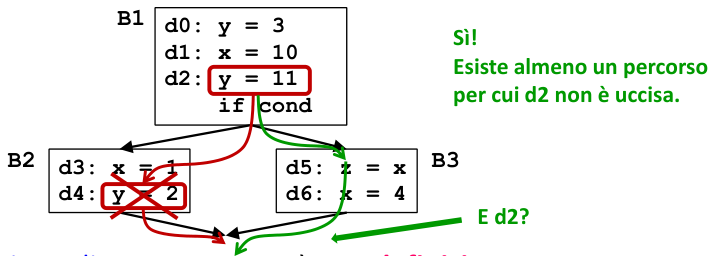
\includegraphics[width=.45\textwidth]{dfa_6.png}
\end{example}


\subsubsection{Schema DFA}

\noindent\begin{minipage}[c]{.67\textwidth}
Consideriamo un flow graph:
\begin{itemize}
  \item aggiungiamo un \textbf{BB entry} e uno \textbf{exit} $\rightarrow$ garantisco \textit{single-entry} e \textit{single-exit} points
  \item per stabilire l'effetto del codice \textbf{in ciascun BB} uso delle \textbf{funzioni di trasferimento} $f_{B}$, che correlano $out[B], in[B]$ per un dato BB $B$
  \item stabilisco l'effetto \textbf{del flusso di controllo} in base alla vicinanza dei blocchi: correlo $out[B_{i}], in[B_{j}]$ di blocchi adiacenti
  \item infine dobbiamo solo risolvere le equazioni 
\end{itemize}
\end{minipage}
\hfill
\begin{minipage}[c]{.3\textwidth}
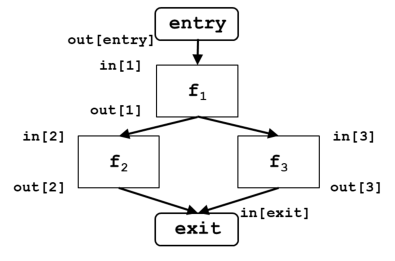
\includegraphics[width=\textwidth]{dfa_7.png}
\end{minipage}

\vspace{-1em}
\begin{emphasize}
    Nota: stabiliamo anche una cosiddetta \textbf{boundary condition}, ovvero qual \`e l'informazione che riceve il primo BB dall'\textit{entry block} $\rightarrow$ per le Reaching Definitions stabiliamo $out[entry] = \emptyset$
\end{emphasize}


\subsubsection{Effetti di uno statement}

\begin{itemize}
  \item la fz.~di trasferimento di uno statement astrae l'esecuzione rispetto al problema di interesse
  \item per uno statement $s$ (\lstinline|d: x = y + z|):
  \begin{itemize}
    \item $Gen[s]$: definizioni \textbf{generate} ($Gen[s] = \lbrace\texttt{d}\rbrace$)
    \item definizioni \textbf{propagate}: $in[s] - Kill[s]$ dove $Kill[s]$ sono le altre definizioni di \lstinline|x| nel resto del programma
    \item funzione di trasferimento di uno statement $s$:
    \begin{equation*}
      out[s] = f_{s}(in[s]) = Gen[s] \cup (in[s] - Kill[s]) 
    \end{equation*}
    
  \end{itemize}
  
  \item in altre parole, $Gen$ \`e l'insieme di propriet\`a \textbf{generate} dal blocco, $Kill$ l'insieme di quelle \textbf{eliminate} nel blocco e $in$ l'insieme di quelle \textbf{ereditate}
  \begin{emphasize}
      Stiamo lavorando su bit vector $\rightarrow$ una $f_{s}$ riempie $out[s]$ a partire da $in[s]$ e applicando qualche tipo di calcolo
  \end{emphasize}
\end{itemize}

\vspace{-2em}
\subsubsection{Effetti di un BB}

\begin{itemize}
  \item la fz.~di trasferimento di un BB compone linearmente le fz.~dei suoi \textit{statements}
    \begin{equation*}
      \begin{split}
        \boxed{out[B]} = f_{B}(in[B]) &= f_{dn}\cdot\ldots\cdot f_{d0} \\
                                      &= \boxed{Gen[B] \cup (in[B] - Kill[B])}
      \end{split}
    \end{equation*}
    \begin{itemize}
      \item $Gen[B]$: definizioni localmente disponibili (\textbf{a fine BB})
      \item $Kill[B]$: definizioni uccise da B \textbf{in tutto il programma}
    \end{itemize}
  \item una $f_{B}$ associa \textbf{incoming reaching definitions} $\rightarrow$ \textbf{outgoing reaching definitions}
\end{itemize}

\vspace{-1em}
\begin{example}
  \begin{center}
    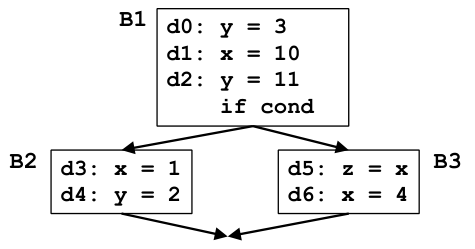
\includegraphics[width=.35\textwidth]{dfa_2.png}\hfill
    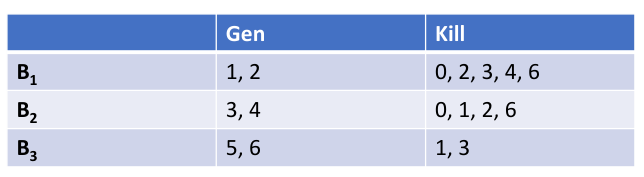
\includegraphics[width=.55\textwidth]{dfa_8.png}
  \end{center}
  \begin{emphasize}
    NB: in $Kill[B1]$ \lstinline|d0| e \lstinline|d2| si uccidono a vicenda $\rightarrow$ l'approccio bit-vector \textbf{non ha nozione di ordine di esecuzione}
  \end{emphasize}
\end{example}

\vspace{-1em}
\subsubsection{Effetti degli archi aciclici}

In caso di predecessori multipli, devo decidere con che criterio unire l'informazione:
\begin{itemize}
  \item nodo di unione (\textbf{join}): nodo con \textbf{predecessori} multipli
  \item operatore di \textbf{meet} ($\wedge$): $in[B] = out[p_1] \cup \ldots \cup out[p_n]$ con $p_1,\ldots,p_n$ tutti predecessori di $B$
  \begin{emphasize}
    Il meet operator \`e \textbf{specifico del problema}, non dell'analisi mediante DFA!
    \noindent $\rightarrow$ Per il problema delle reaching definitions, usiamo $\wedge = \cup$ in quanto la condizione deve essere verificata per \textit{almeno un percorso}
  \end{emphasize}
\end{itemize}

\begin{figure}[h]
  \centering
  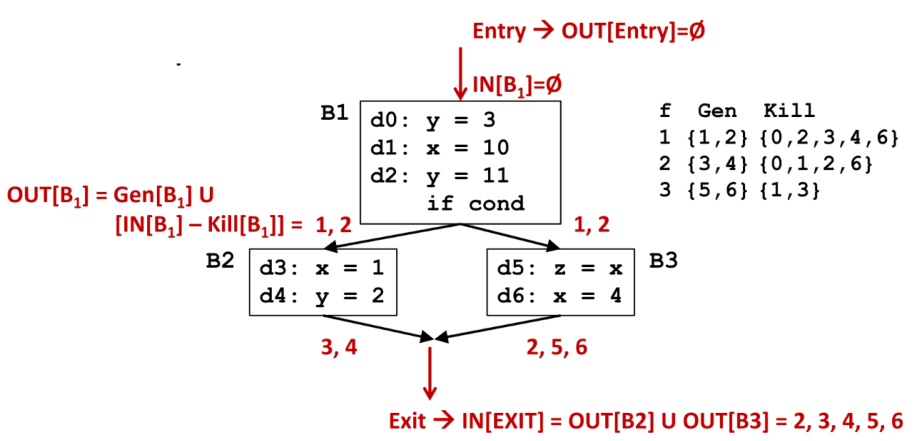
\includegraphics[width=.65\textwidth]{dfa_9.png}
  \caption{Esempio (continua)}
\end{figure}

\subsubsection{Effetti degli archi ciclici e condizioni iniziali}

Gli archi ciclici (\textit{backedges}) possono cambiare le loro $out$ o non averle ancora calcolate durante l'esecuzione dell'algoritmo:
\begin{itemize}
  \item \textbf{itero fino a convergenza}
  \item definisco delle \textbf{condizioni iniziali} per inizializzare ogni BB (similmente alla boundary condition): stabilisco $out[B] = \emptyset$ (specifico per Reaching Defs.)
\end{itemize}

\subsubsection{Algoritmo iterativo}

\begin{lstlisting}
input: control flow graph CFG = (N, E, Entry, Exit)
// Boundary condition
  out[Entry] = $\emptyset$

// Initialization for iterative algorithm
  for each basic block B other than Entry
    out[B] = $\emptyset$

// Iterate
  while (changes to any out[] occur) {
    in[B] = $\cup$ (out[p]), for all predecessors p of B
    out[B] = f$_B$(in[B])   // $\textcolor{codeblue}{out[B] = Gen[B] \cup (in[B] - Kill[B])}$
  }\end{lstlisting}

\begin{example}[frametitle={Esempio di eseguzione}]
    \noindent\begin{minipage}[c]{.45\textwidth}
    \begin{emphasize-blue}
      La rappresentazione del bit-vector segue l'ordine di numerazione delle definizioni: \lstinline|IN[B1] = <000 00 0 0>| con \lstinline|d1| primo bit, ...
    \end{emphasize-blue}
    
    Nota: dopo la seconda iterazione $out[B2]$ non cambia pi\`u
    \end{minipage}
  \begin{minipage}[c]{.55\textwidth}
  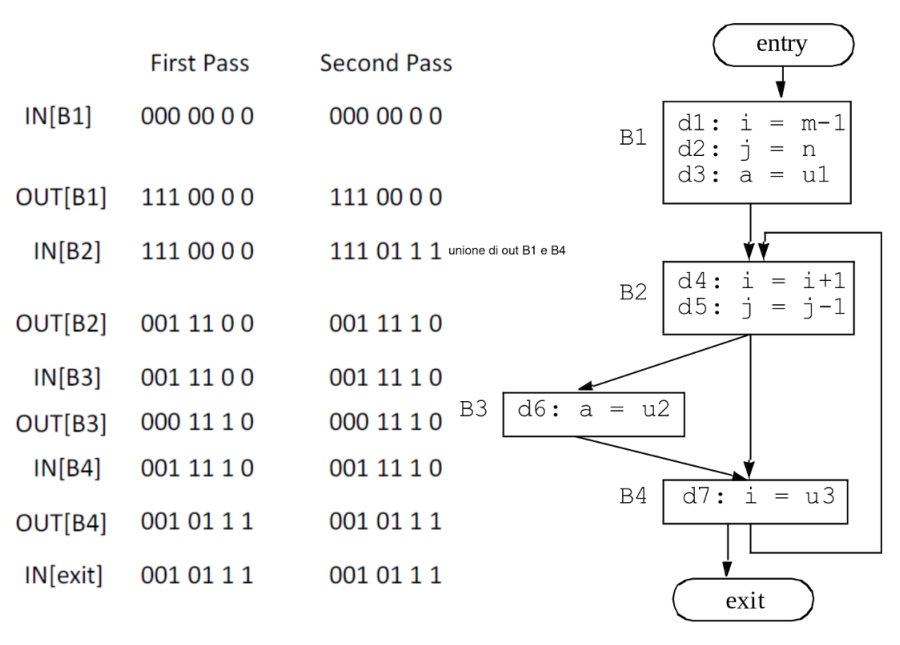
\includegraphics[width=\textwidth]{dfa_10.png}
  \end{minipage}
\end{example}

\subsubsection{Algoritmo Worklist}

La worklist contiene le variabili che devono ancora essere processate. Quando la worklist \`e vuota l'algoritmo termina.
  
\begin{lstlisting}
input: control flow graph CFG = (N, E, Entry, Exit)

// Initialize
  out[Entry] = $\emptyset$  // can set out[Entry] to special def
                  // if reaching then undefined use
  for all nodes i
    out[i] = $\emptyset$    // can optimize by out[i] = gen[i]
  ChangedNodes = N

// Iterate
  while ChangedNodes $\neq \emptyset$ {
  remove i from ChangedNodes
  in[i] = $\cup$ (out[p]), for all predecessors p of i
  oldout = out[i]
  out[i] = f$_i$(in[i])     // $\textcolor{codeblue}{out[B] = Gen[B] \cup (in[B] - Kill[B])}$
  if (oldout $\neq$ out[i]){
    for all successors s of i
      add s to ChangedNodes
  }
}\end{lstlisting}

\subsection{Liveness Analysis}

\subsubsection{Live Variable Analysis}

\noindent\begin{minipage}[c]{.7\textwidth}
\paragraph{Definizione:}

Una variabile \lstinline|v| \`e \textbf{viva} (\textit{live}) in un punto \textit{p} del programma se il valore di \lstinline|v| \`e usato lungo qualche percorso del FG a partire da \textit{p} (altrimenti \`e \textbf{morta})\\

\paragraph{Motivi dell'analisi:}

(oltre alla DCE) es. \textit{register allocation}: i registri reali sono limitati - la \textit{ra} \`e l'operazione che cerca di evitare le spill in cache e in memoria, cercando i casi in cui risulta possibile \textbf{riutilizzare} un certo registro $\rightarrow$ dipende evidentemente dalla liveness di una variabile\\

\paragraph{Definizione del problema DFA}

\begin{itemize}
  \item devo stabilire $\forall$ BB quali sono le variabili \textbf{vive} in ciascuno di essi
  \item bit-vector di lunghezza pari al numero di variabili
\end{itemize}
\end{minipage}
\begin{minipage}[c]{.3\textwidth}
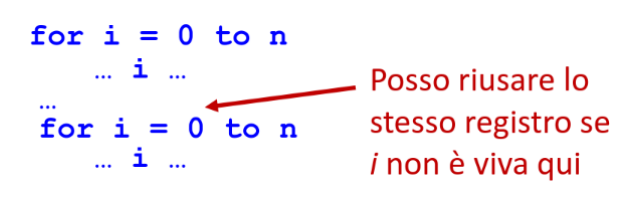
\includegraphics[width=\textwidth]{dfa_11.png}
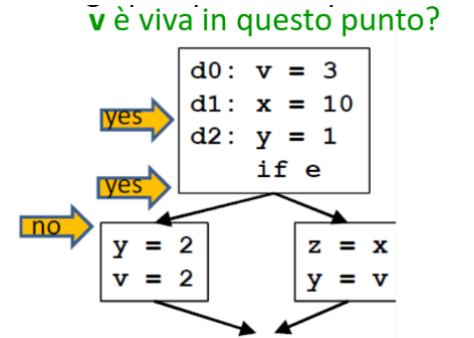
\includegraphics[width=\textwidth]{dfa_12.png}
\end{minipage}

\subsubsection{Forward e Backward analysis}

es.~\textit{Reaching Definitions}: che informazione sto cercando per capire se una definizione raggiunge o meno un punto \textit{p} del programma? Devo analizzare il "\textbf{passato}" - gli statement tra la definizione e \textit{p} per cercare eventuali kill (analizzo da \textit{entry} a \textit{p})

\noindent $\rightarrow$ Nel contesto della \textit{Liveness Analysis} invece, devo analizzare il "\textbf{futuro}" - cerco gli usi della variabile da \textit{exit} a \textit{p}

\subsubsection{Funzione di trasferimento}

Per la formulazione pi\`u tipica della \textit{LA} (ce ne sono diverse, a seconda delle fonti) usiamo
\begin{itemize}
  \item l'insieme delle variabili vive che pu\`o \textbf{generare} un BB ($Use[B]$)
  \item l'insieme delle variabili \textbf{definite} nel BB ($Def[B]$)
  \item le variabili vive in ingresso che il bb pu\`o propagare ($Out[B] - Def[B]$)
  \item[$\rightarrow$] \textbf{funzione di trasferimento} per il blocco $B$:
  \begin{equation*}
    In[B] = Use[B] \cup (Out[B] Def[B]) 
  \end{equation*}
\end{itemize}

\paragraph{Flow Graph}

\begin{itemize}
  \item $In[B] = f(Out[B])$ (\textit{backward analysis}, contrario rispetto a \textit{Reaching Definitions})
  \item \textbf{join} node: nodo con \textbf{successori} multipli
  \item \textbf{meet} operator ($\wedge$): $out[B] = in[s_1] \cup \ldots \cup in[s_n]$ con $s_1,\ldots,s_n$ tutti predecessori di $B$\\
    (ricorda: $\cup \implies \exists$ almeno un percorso)
\end{itemize}

\subsubsection{Algoritmo iterativo}

\noindent\begin{minipage}[c]{.3\textwidth}
\begin{itemize}
  \item \textbf{boundary condition}: $\emptyset$
  \item \textbf{starting conditions}: $\emptyset$
\end{itemize}
\end{minipage}\hfill
\begin{minipage}[c]{.67\textwidth}
\begin{emphasize}
  La scelta delle condizioni iniziali deriva principalmente dalla scelta del meet operator - se per qualsiasi motivo scegliessimo come meet operator $\cap$, usare $\emptyset$ impedirebbe qualsiasi propagazione dell'informazione
\end{emphasize}
\end{minipage}

\vspace{1em}
\begin{lstlisting}
input: control flow graph CFG = (N, E, Entry, Exit)

// Boundary condition
  in[Exit] = $\emptyset$

// Initialization for iterative algorithm
  for each basic block B other than Exit
    in[B] = $\emptyset$

// Iterate
  while (changes to any in[] occur) {
    for each basic block B other than Exit {
      out[B] = $\cup$ (in[s]), for all successors s of B
      in[B] = f$_B$(out[B])   // $\textcolor{codeblue}{in[B] = Use[B] \cup (Out[B] - Def[B])}$
    }
}\end{lstlisting}

\begin{emphasize}
  A convergenza si arriva \textbf{indipendentemente dall'ordine} in cui calcolo le funzioni dei BB (cambia al massimo il numero di iterazioni per arrivarci)
\end{emphasize}

\begin{example}
  \begin{center}
    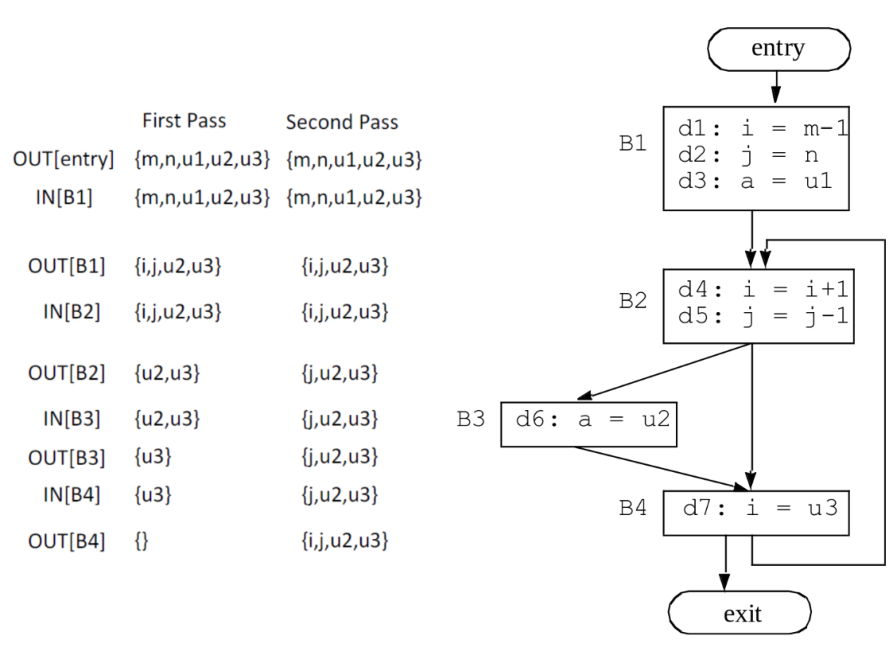
\includegraphics[width=.5\textwidth]{dfa_13.png}
  \end{center}
\end{example}

\subsection{Framework per DFA}

Possiamo usare una tabella di questo tipo per descrivere problemi nell'ambito della DFA:

\begin{center}
  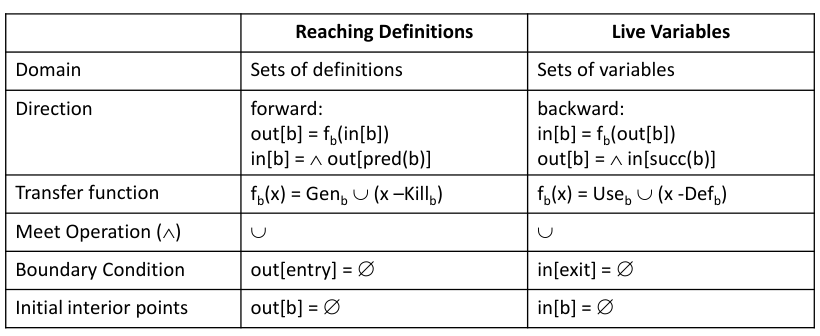
\includegraphics[width=.65\textwidth]{dfa_14.png}
\end{center}

\subsection{Available Expressions}

Altro problema modellabile tramite DFA, utile ad es.~per la Common Subexpression Elimination

\begin{center}
  \begin{minipage}[c]{.4\textwidth}
    \begin{lstlisting}[linewidth=.6\linewidth]
  if (...) {
    x = m + n;
  } else {
    y = m + n;
  }
    z = m + n;\end{lstlisting}
    \lstinline|m + n| \`e ridondante perch\'e gi\`a calcolato
  \end{minipage}\quad
  \begin{minipage}[c]{.5\textwidth}
    \begin{lstlisting}[linewidth=.48\linewidth]
  if (...) {
    x = m + n;
  } else {
    ...
  }
    z = m + n;\end{lstlisting}
    Cosa cambia se non viene calcolato nel ramo \lstinline|else|?
  \end{minipage}
\end{center}

Il concetto di available expr.~\`e necessario come maniera rigorosa di ragionare sulla \textbf{ridondanza}

\paragraph{Definizione del problema:}

\begin{itemize}
  \item \textbf{dominio}: tutte le espressioni del programma
    \begin{itemize}
      \item consideriamo solo espr.~binarie del tipo $x \oplus y$
    \end{itemize}
  \item un'espressione $x \oplus y$ \`e \textbf{available} in un punto \textit{p} del programma se \textbf{ogni} percorso che parte da \textit{Entry} e arriva a \textit{p} valuta l'espressione
  \item \textbf{funzione di trasferimento} di un BB:
    \begin{equation*}
      f_{B}(x) = Gen[B] \cup (x - Kill[B])
    \end{equation*}
    \begin{itemize}
      \item un blocco \textbf{genera} l'espressione $x \oplus y$ se la valuta e \textbf{non ridefinisce in seguito} \textit{x} o \textit{y}
      \item un blocco \textbf{uccide} l'espr. $x \oplus y$ se assegna (o potrebbe assegnare) un valore a \textit{x} o \textit{y} e non ricalcola successivamente l'espressione
    \end{itemize}
  \item \textbf{direzione di analisi}: \textbf{forward}
    \begin{itemize}
      \item nell'analisi delle \textit{Available Expressions} eliminiamo un'espr.~perch\'e \`e stata calcolata \textbf{in passato}
      \item (nell'analisi delle \textit{Live Variables} eliminiamo una var.~perch\'e non verr\`a usata \textbf{in futuro})
    \end{itemize}
  \item equazioni $Out$: $Out[B] = f_{b}(In[B])$
  \item equazioni $In$: $In[B] = \wedge _{p\in pred(B)}(Out[B])$
  \item \textbf{meet} operator ($\wedge$): $\cap$ ("\textbf{ogni percorso} che parte da Entry [...]")
    \begin{center}
      
\includegraphics[width=.5\textwidth]{dfa_15.png}
    \end{center}
\end{itemize}

\noindent\begin{minipage}[c]{.5\textwidth}
\begin{itemize}
  \item \textbf{boundary conditions}: $Out[Entry] = \emptyset$
  \item \textbf{initial conditions}:
    \begin{itemize}
      \item $\textcolor{red}{\xcancel{\textcolor{black}{Out[B_{i}] = \emptyset}}}$ $\rightarrow$ il meet op.~\`e $\cap$
      \item $Out[B_{i}] = \mathcal{U}$
    \end{itemize}
\end{itemize}
\end{minipage}\hfill
\begin{minipage}[c]{.4\textwidth}
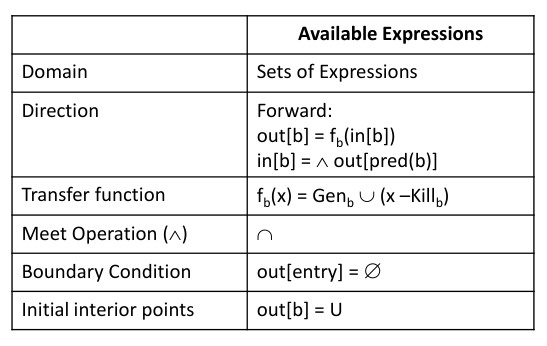
\includegraphics[width=\textwidth]{dfa_17.png}
\captionof{figure}{Tabella completa}
\end{minipage}

\begin{example}
\noindent\begin{minipage}[c]{.65\textwidth}
  Risolto su fogli, dominio $\lbrace$\lstinline|a=b,a*b,a-1|$\rbrace$
\begin{emphasize}
  Essendo la DFA per natura \textbf{statica}, considera sempre il caso \textbf{peggiore} di esecuzione.\\
  Il risultato dell'analisi sarebbe diverso se conoscessi l'istanza specifica - sapendo ad es.~che BB4 sar\`a falso potrei fare delle assunzioni che, staticamente, non posso fare $\rightarrow$ ritorno conservativamente al caso peggiore che il loop esegua almeno una volta
\end{emphasize}
\end{minipage}\hfill
\begin{minipage}[c]{.3\textwidth}
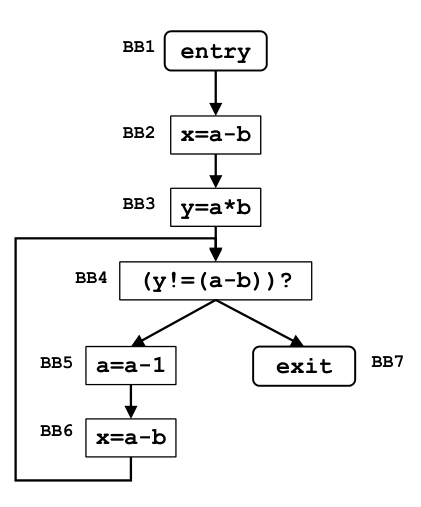
\includegraphics[width=\textwidth]{dfa_16.png}
\end{minipage}
\end{example}

\section{Loops e UD-DU chains}

\subsection{Cos'\`e un loop}

Sapendo che un programma spende la maggior parte del tempo nei loop, l'obiettivo \`e definire un loop \textbf{in termini di teoria dei grafi} (CFG), ovvero \textbf{indipendentemente dalla loro sintassi e dal tipo} (\lstinline|for|, \lstinline|while|, \lstinline|goto|, costrutti stile assembly con salti condizionati e non...)\\

\noindent\begin{minipage}[c]{.45\textwidth}
\textbf{Elementi chiave per riconoscere un loop}:
\begin{itemize}
  \item gli archi devono formare almeno un ciclo
  \item (fondamentale) \textbf{singolo entry point} (tutti gli archi, se multipli, devono entrare nello stesso punto)
\end{itemize}
\end{minipage}\hfill
\begin{minipage}[c]{.5\textwidth}
\begin{example}[frametitle={}]
  \noindent\begin{minipage}[c]{.7\textwidth}
    Generalmente, non tutti i \textit{cicli} sono un "loop" da un p.to di vista dell'ottimizzazione: $\textcolor{red}{c\rightarrow d}$ \`e un loop, $\textcolor{blue}{a\rightarrow c \rightarrow d}$ no
  \end{minipage}\hfill
  \begin{minipage}[c]{.25\textwidth}
  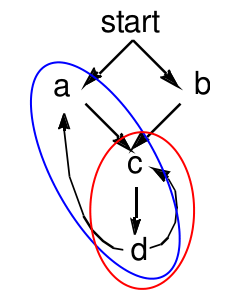
\includegraphics[width=\textwidth]{uddu_1.png}
  \end{minipage}
\end{example}
\end{minipage}

\subsubsection{Definizioni formali}

\paragraph{Dominator}

Un nodo \textit{d} domina un nodo \textit{n} in un grafo ( \textit{d dom n} ) se ogni percorso da \textit{ENTRY} a \textit{n} passa per \textit{d}
\paragraph{Immediate dominator}

L'\textbf{ultimo dominator} di \textit{n} su qualsiasi percorso da \textit{ENTRY} a \textit{n}

\textit{m} domina \textbf{immediatamente} (strettamente) \textit{n} (\textit{m sdom n}) $\iff$ $m\, dom \,n\land m \neq n$

\paragraph{Dominator Tree}

Modo per rappresentare la propriet\`a di dominanza \textbf{in forma di albero}

\begin{itemize}
  \item $a \rightarrow b$ nel dominator tree $\iff$ \textit{a sdom b}
  \item \textbf{non compaiono} le relazioni di \textbf{"auto-dominazione"} (ogni nodo domina sempre se stesso, ma nell'albero non serve rappresentarlo)
  \item \textit{ENTRY} \`e la \textbf{radice}
  \item ogni nodo \textit{d} domina solo \textbf{i suoi discendenti} nell'albero
\end{itemize}

\begin{example}[frametitle={Esempi di DT}]
   \begin{minipage}[c]{.24\textwidth}
   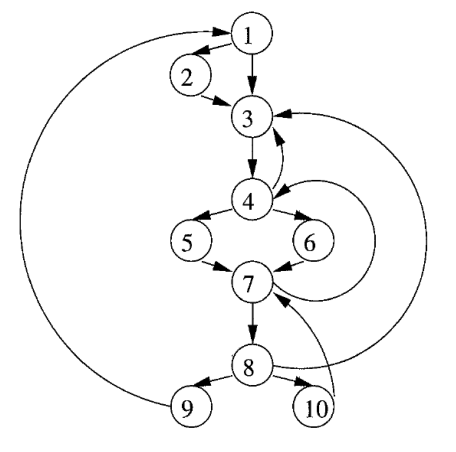
\includegraphics[width=\textwidth]{uddu_2.png}
   \end{minipage}
   \begin{minipage}[c]{.24\textwidth}
   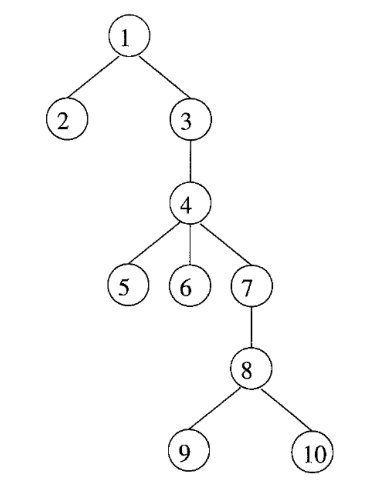
\includegraphics[width=\textwidth]{uddu_3.png}
   \end{minipage}\hfill\vline\hfill
   \begin{minipage}[c]{.48\textwidth}
   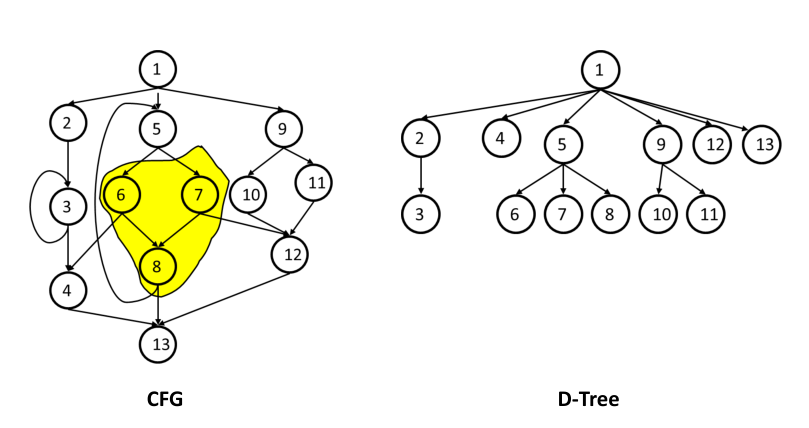
\includegraphics[width=\textwidth]{uddu_4.png}
   \label{example-dt}
   \end{minipage}
\end{example}


\subsubsection{Loop naturali}

Nonostante le diverse forme trovate nei sorgenti, dal punto di vista dell'analisi ci interessa solo che abbiano propriet\`a che facilitino l'ottimizzazione, ovvero
\begin{itemize}
  \item \textbf{singolo entry point}: header $\rightarrow$ l'header \textbf{domina tutti i nodi nel loop}
  \item back edge, ossia arco la cui testa domina la propria coda (tail $\rightarrow$ head): un back edge \textbf{deve far parte di almeno un loop}
\end{itemize}

\subsection{Identificare i loop naturali}

\begin{enumerate}
  \item trovare le relazioni di \textbf{dominanza}
  \item identificare i \textbf{back edges}
  \item trovare il \textbf{loop naturale associato} al back edge
\end{enumerate}

\subsubsection{Trovare i dominatori}

Lo impostiamo in termini di DFA (vedi secondo assignment)

\subsubsection{Trovare i back edges}

\noindent \begin{minipage}[c]{.67\textwidth}
Usiamo un algoritmo basato su \textit{depth-first traversal
}
\begin{itemize}
  \item inizio alla radice e visito \textbf{ricorsivamente} i figli di ogni nodo \textbf{in qualsiasi ordine}
  \item importante la "velocit\`a di discesa": prima scendo ed esploro \textbf{in profondit\`a}, a prescindere dall'ordine
\end{itemize}

Il percorso della visita definisce un \textbf{depth-first spanning tree (DFST)}:
\begin{itemize}
  \item archi \textbf{solidi}: struttura del DT
  \item archi \textbf{tratteggiati}: altri archi del CFG
\end{itemize}
\end{minipage}\hfill
\begin{minipage}[c]{.3\textwidth}
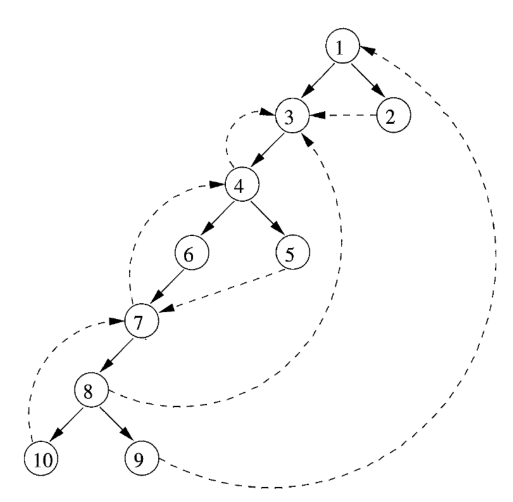
\includegraphics[width=\textwidth]{uddu_5.png}
\end{minipage}

\paragraph{Categorizzazione degli archi}

\begin{itemize}
  \item \textbf{advancing} (A) edges: da antenato a discendente, ovvero gli archi detti \textit{proper} - gli archi solidi sono tutti A
  \item \textbf{retreating} (R) e.: da discendente a antenato (non necessariamente proper $\rightarrow$ da un nodo a se stesso) - solo archi tratteggiati
  \item \textbf{cross} (C) e.: archi tali per cui nessuno dei due nodi \`e antenato dell'altro
\end{itemize}

\begin{emphasize}
    Se disegniamo il DFST in modo che i figli siano aggiunti da sx a dx nell'ordine di visita, allora i cross edges vanno sempre da dx a sx
\end{emphasize}

\noindent \begin{minipage}[c]{.67\textwidth}
\paragraph{Algoritmo}

\begin{itemize}
  \item esegui una depth-first search
  \item $\forall$ retreating edge $t \rightarrow h$ controlla se \textit{h dom t}
\end{itemize}


\begin{emphasize}
  Vado a riconoscere i \textit{back edges} come casi specifici di \textit{retreating edges} $\rightarrow$ la maggior parte dei programmi hanno control flow \textbf{riducibili}, ovvero tutti i \textit{retreating edges} sono anche back
\end{emphasize}
\end{minipage}\hfill
\begin{minipage}[c]{.3\textwidth}
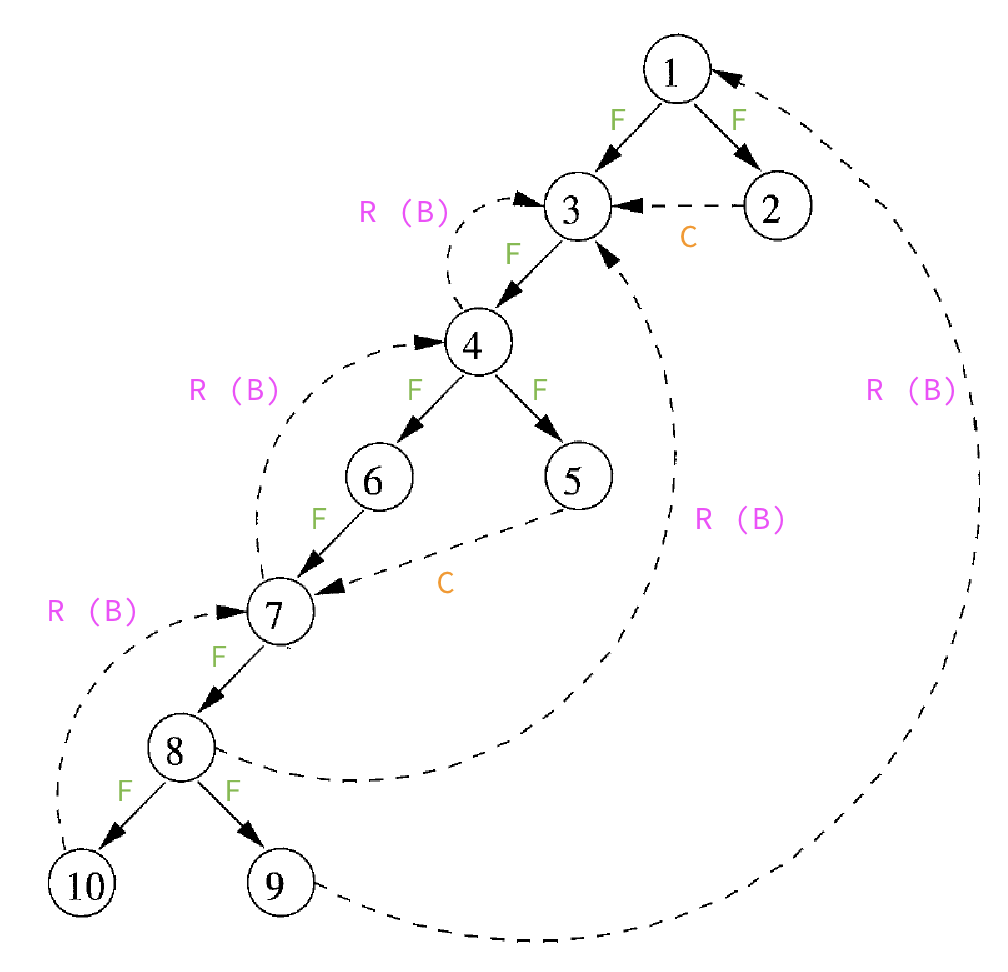
\includegraphics[width=\textwidth]{uddu_5b.png}
\end{minipage}

\subsubsection{Trovare il loop naturale associato}

Il loop naturale di un back edge \`e il \textbf{pi\`u piccolo} insieme di nodi che \textbf{include head e tail} del back edge e \textbf{non ha predecessori fuori da questo insieme} 

\paragraph{Algoritmo}
\begin{itemize}
  \item eliminare \textit{h} dal CFG
  \item trovare i nodi che raggiungono \textit{t}: questi (pi\`u \textit{h}) formano il \textbf{loop naturale} $t \rightarrow h$
\end{itemize}


$\rightarrow$ genericamente rappresento i loop in maniera "header-centrica"

\subsection{Preheader}

\noindent\begin{minipage}[c]{.65\textwidth}
Spesso (propedeutico a varie ott.) \`e necessario garantire che, quando arrivo all'header, ci arrivo tramite arco \textit{fallthrough}: es.~LICM (caso di code hoisting), che sposta un'istr.~in un punto comune al control flow di tutte le iterazioni del loop\\
$\rightarrow$ tipicamente inserisco un blocco \textit{preheader} appena prima del loop, apposta per inserire le istr.~"hoistate"
\end{minipage}\hfill
\begin{minipage}[c]{.3\textwidth}
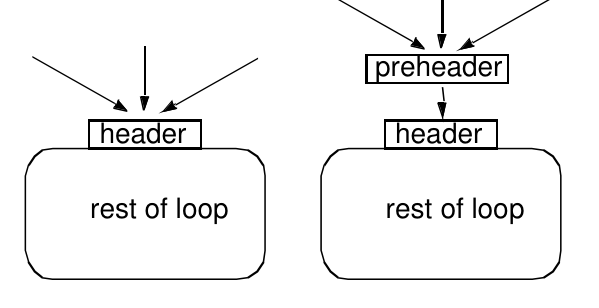
\includegraphics[width=\textwidth]{uddu_6.png}
\end{minipage}

\begin{emphasize}
  Per manipolare i loop in LLVM esistono primitive per recuperare proprio questi blocchi fondamentali (poi per navigare nel resto dei BB usiamo gli iteratori, sia seguendo l'ordine del CFG sia non)
\end{emphasize}

\subsection{Use-def e Def-use chains}

La capacit\`a di ricollegare in maniera efficiente la definizione di una variabile a tutti i suoi usi (per esempio per propagare un risultato) \`e indispensabile all'ottimizzazione $\rightarrow$ per questo vengono previsti questi riferimenti nell'IR LLVM

\subsubsection{Dove viene definita o usata una variabile}

Le definizioni di DU e UD chain \textbf{precedono quella di SSA} $\rightarrow$ lo scope lessicale del programma in cui si potevano trovare gli usi della variabile era molto pi\`u ampio

\begin{example}[frametitle={Esempi}]
  \noindent 
  \begin{minipage}[c]{.65\textwidth}
    \begin{itemize}
      \item LICM: se le var.~usate nell'espressione che definisce \lstinline|A| sono \textbf{definite all'interno del loop}, non posso spostare la definizione fuori
      \item CP: per un dato uso di \lstinline|X|, trovo le sue \textit{reaching definitions} (es.~\lstinline|X = Y|) e, se non sono ridefinite (appunto "reaching") vado a sostituirne gli usi
    \end{itemize}

  \end{minipage}\hfill
  \begin{minipage}[c]{.25\textwidth}
    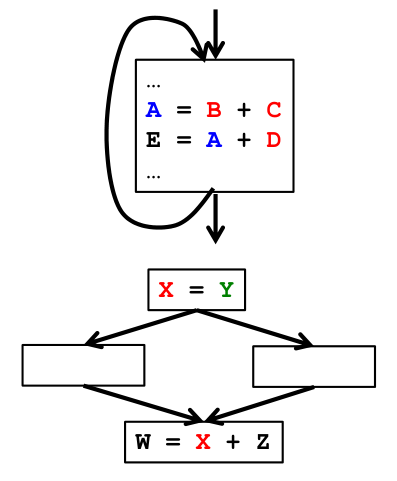
\includegraphics[width=\textwidth]{uddu_7.png}
  \end{minipage}

\noindent A questo tipo di ottimizzazioni beneficia molto poter scorrere agevolmente le relazioni DU delle variabili $\rightarrow$ vogliamo un'IR che lo preveda e dunque permetta una \textbf{forma di analisi "sparsa"} (ignoro tutte le istruzioni non relative alla var.~correntemente analizzata)
\end{example}

In generale le catene possono essere onerose (per $N$ defs e $M$ uses, $O(NM)$ spazio e tempo) $\rightarrow$ Possiamo semplificare ulteriormente se riusciamo a \textbf{ridefinire completamente anche il nome della variabile ad ogni sua ridefinizione} (ci avviciniamo a SSA) (permette catene sensibilmente pi\`u corte)

\noindent\begin{minipage}[b]{.45\textwidth}
  \centering
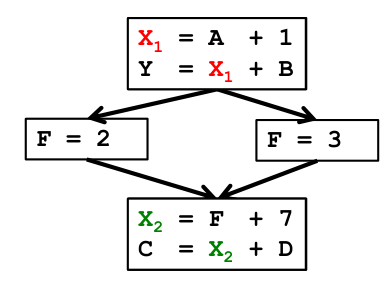
\includegraphics[width=.65\textwidth]{uddu_8.png}
\captionof{figure}{Un altro motivo per rinominare le ridefinizioni \`e che occorrenze della stessa variabile potrebbero essere scorrelate e dunque ottimizzabili separatamente}
\end{minipage}\hfill
\begin{minipage}[b]{.5\textwidth}
  \centering
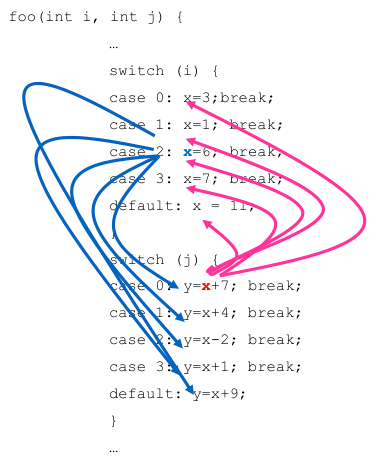
\includegraphics[width=.65\textwidth]{uddu_9.png}
\captionof{figure}{Esempio di catena onerosa. Ulteriore soluzione \`e \underline{limitare ogni variabile a una definizione}}
\end{minipage}

\section{Static Single Assignment (SSA)}

\noindent\begin{minipage}[t]{.4\textwidth}
  \vspace{.5em}
Forma di IR dove ad ogni variabile viene \textbf{assegnato un valore solo una volta}\\ $\rightarrow$ Facile dentro ad un BB, ma cosa succede nei punti di \textbf{join} di un CFG?\\
$\rightarrow$ \textbf{usiamo una notazione fittizia: la $\Phi$ function}
\end{minipage}\hfill
\begin{minipage}[t]{.58\textwidth}
\begin{example}[frametitle={Local value numbering}]
  \begin{center}
    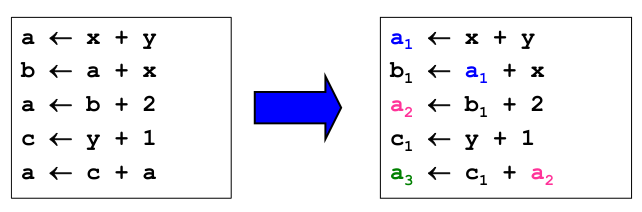
\includegraphics[width=\textwidth]{uddu_10.png}
  \end{center}

    All'interno di un BB posso fare \textit{local value numbering}, visitando ogni istruzione in ordine:
    \begin{itemize}
      \item LHS: assegna ad una nuova versione della variabile
      \item RHS: usa la versione pi\`u recente della stessa
    \end{itemize}

\end{example}
\end{minipage}

\noindent\begin{minipage}[c]{.4\textwidth}
\begin{lstlisting}
c $\leftarrow$ 12
if (i) {
  a $\leftarrow$ x + y
  b $\leftarrow$ a + x
} else {
  a $\leftarrow$ b + 2
  c $\leftarrow$ y + 1
}
a $\leftarrow$ c + a\end{lstlisting}
\end{minipage} \hfill $\rightarrow$ \hfill
\begin{minipage}[c]{.4\textwidth}
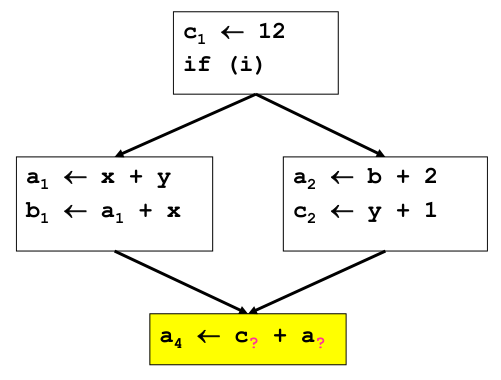
\includegraphics[width=\textwidth]{uddu_10b.png}
\end{minipage}

\subsection{La funzione $\Phi$}

\noindent\begin{minipage}[c]{.65\textwidth}
\begin{itemize}
  \item $\Phi$ fonde multiple definizioni derivanti da multipli percorsi in una singola definizione
  \item per un BB con \textit{p} predecessori ci sono \textit{p} argomenti nella funzione $\Phi$:
  \begin{lstlisting}
xnew $\leftarrow \Phi$(x1, x2, ..., xp)\end{lstlisting}
\item tipicamente \textbf{non ci interessa quale \lstinline|xi| usare} $\rightarrow$ se rilevante, usiamo le definizioni derivanti dall'arco di interesse
\end{itemize}
\end{minipage}\hfill
\begin{minipage}[c]{.3\textwidth}
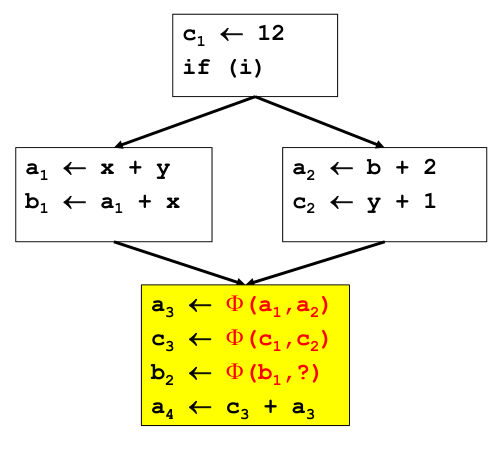
\includegraphics[width=\textwidth]{uddu_11.png}
\end{minipage}

\begin{example}[frametitle={Come si implementa $\Phi$}]
  \noindent \begin{minipage}[c]{.5\textwidth}
    Di fatto, a tempo di esecuzione ci sar\`a sempre un percorso \textbf{effettivamente eseguito} $\rightarrow$ per questo consideriamo $\Phi$ come notazione fittizia
  \end{minipage}\hfill
  \begin{minipage}[c]{.3\textwidth}
    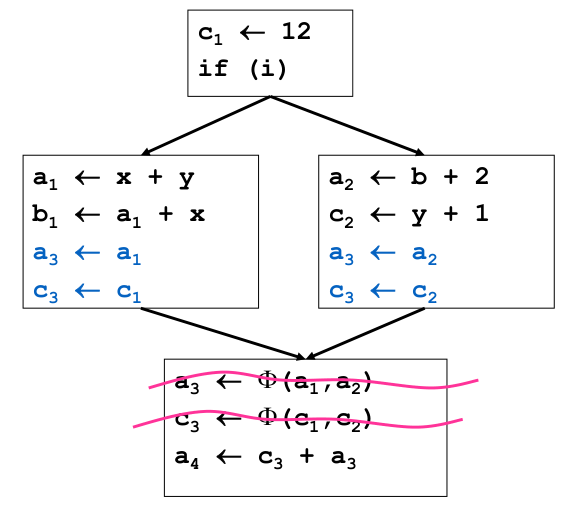
\includegraphics[width=\textwidth]{uddu_12.png}
  \end{minipage}
\end{example}

\subsection{SSA triviale}

\noindent \begin{minipage}[c]{.4\textwidth}
\begin{itemize}
  \item ogni assegnamento genera una nuova versione della variabile
  \item aggiungiamo una fz.~$\Phi$ \textbf{ad ogni p.to di join $\forall$ le variabili \textit{live}}  
\end{itemize}
\end{minipage}\hfill
\begin{minipage}[c]{.55\textwidth}
  \centering
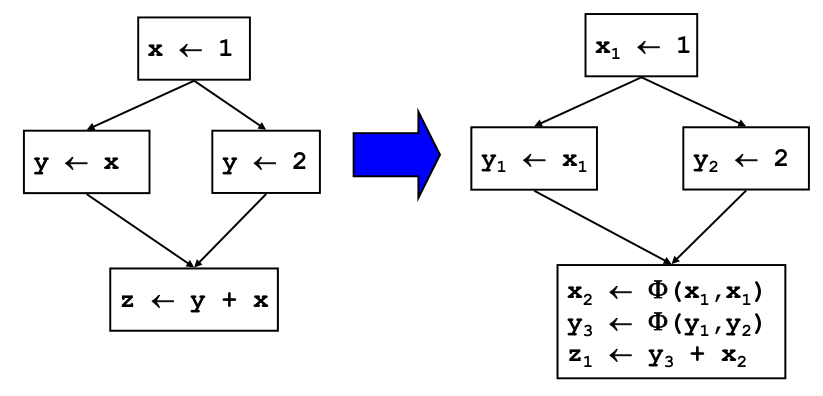
\includegraphics[width=.7\textwidth]{uddu_13.png}
\captionof{figure}{Molte di queste funzioni $\Phi$ non sono necessarie}
\end{minipage}

\subsection{SSA minimale}

\noindent \begin{minipage}[c]{.6\textwidth}
\begin{itemize}
  \item ogni assegnamento genera una nuova versione della variabile
  \item aggiungiamo una fz.~$\Phi$ ad ogni p.to di join $\forall$ le variabili \textit{live} \textbf{con definizioni multiple} 
\end{itemize}
\end{minipage}\hfill
\begin{minipage}[c]{.25\textwidth}
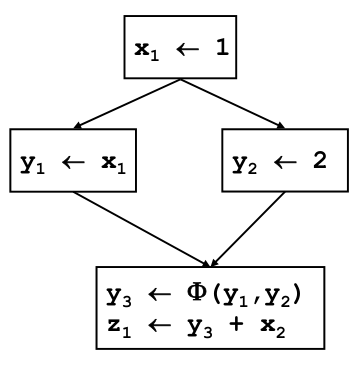
\includegraphics[width=\textwidth]{uddu_14.png}
\end{minipage}

\begin{example}[frametitle={Esempio con loop}]
  \noindent\begin{minipage}[c]{.5\textwidth}
  \lstinline|c1| altro non \`e che la rappresentazione del valore iniziale che assume \lstinline|c| a tempo del primo assegnamento (prima esecuzione del loop), mentre \lstinline|c2| il valore della variabile all'iterazione precedente
  \end{minipage}\hfill
  \begin{minipage}[c]{.45\textwidth}
  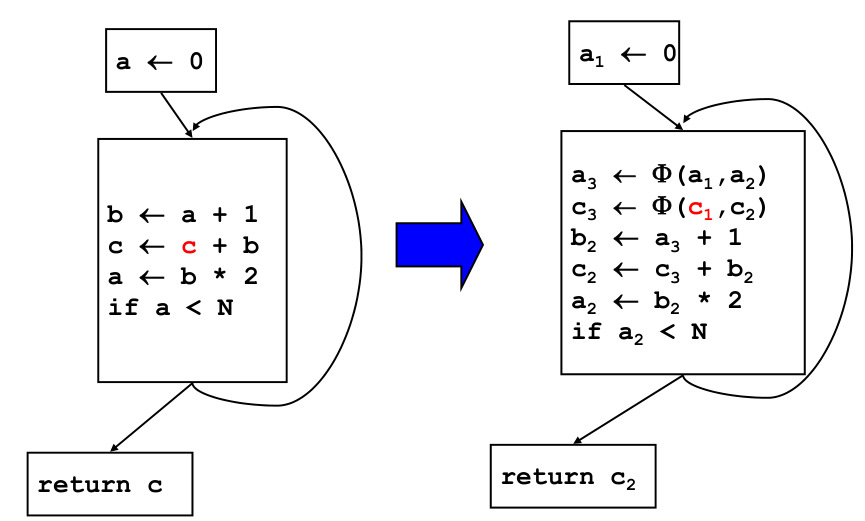
\includegraphics[width=\textwidth]{uddu_15.png}
  \end{minipage}
\end{example}

\subsection{Dove inserire le funzioni $\Phi$}

\noindent \begin{minipage}[c]{.7\textwidth}
Inserisco una $\Phi$ per una variabile \lstinline|a| nel blocco \textit{Z} $\iff$:
\begin{itemize}
  \item \lstinline|a| \`e stata definita pi\`u di una volta (es.~in \textit{X} e \textit{Y}, $X\neq Y$)
  \item $\exists$ due percorsi da \textit{X} a \textit{Z} e da \textit{Y} a \textit{Z} t.c.
  \begin{itemize}
    \item $Pxz \cap Pyz = \left\lbrace Z \right\rbrace$ (\textbf{\textit{Z} unico BB comune} tra i percorsi)
    \item $Z \notin Pxq \lor Z \notin Pyr,\, \text{dove}\, Pxz = Pxq \rightarrow Z, Pyz = Pyr \rightarrow Z$ (almeno un percorso \textbf{raggiunge \textit{Z} per la prima volta})
  \end{itemize}
\end{itemize}
\end{minipage}\hfill
\begin{minipage}[c]{.25\textwidth}
\includegraphics[width=\textwidth]{uddu_17.png}
\end{minipage}

\begin{emphasize}[frametitle={Note}]
  \begin{itemize}
    \item\textit{ENTRY} contiene una definizione implicita di tutte le variabili
    \item\lstinline|v = |$\Phi$\lstinline|(...)| \`e una definizione di \lstinline|v|
\end{itemize}
\end{emphasize}

\subsection{Propriet\`a di dominanza della forma SSA}

Nella forma SSA le \textbf{definizioni dominano gli usi}:
\begin{itemize}
  \item se \lstinline|xi| \`e usato in \lstinline|x| $\leftarrow \Phi$ \lstinline|(..., xi, ...)| $\implies$ BB(\lstinline|xi|) \textbf{domina} il predecessore i-esimo di BB($\Phi$)
  \item se \lstinline|x| \`e usato in \lstinline|y| $\leftarrow$ \lstinline|... x ...| $\implies$ BB(\lstinline|x|) \textbf{domina} BB(\lstinline|y|)
\end{itemize}

SI pu\`o usare questa propriet\`a per derivare un algoritmo efficiente per convertire la IR in forma SSA

\subsection{Dominanza e Dominance Frontier}

Risulta interessante considerare i BB "appena prima" o "appena dopo" i blocchi dominati o che ci dominano $\rightarrow$ i \textbf{dominators} e \textbf{postdominators} ci dicono quale BB \textbf{deve} essere eseguito \textbf{prima}, o \textbf{dopo}, un certo BB \textit{x}\\

\noindent\textbf{Dominance Frontier} di un nodo \textit{x}: $\boxed{DF(x) = \left\lbrace w | x\, dom\, pred(w) \land !(x\, sdom\, w)\right\rbrace}$

\noindent $\rightarrow$ ovvero, l'insieme di tutti i BB che sono successori immediati dei blocchi dominati da \textit{x}, ma che non sono strettamente dominati da \textit{x}

\begin{example}
    \noindent\begin{minipage}[c]{.5\textwidth}
      Per il CFG di esempio, \underline{$DF(5) = \left\lbrace 4,5,12,13 \right\rbrace$}: osservando il DT (pag.~\pageref{example-dt}), notiamo che 4, 12, 13 sono successori di 6, 7, 8 (prima parte della condizione), e non sono dominati da 5 (dunque neppure strettamente, seconda parte). Anche 5 \`e successore di 8, e poich\'e un nodo non domina strettamente se stesso, lo includiamo nella $DF$
    \end{minipage}
    \begin{minipage}[c]{.5\textwidth}
    \includegraphics[width=\textwidth]{uddu_18.png}
    \end{minipage}
\end{example}

\subsection{Utilizzo della Dominance Frontier per calcolare la forma SSA}

I passaggi da seguire sono
\begin{enumerate}
  \item posizionare tutte le funzioni $\Phi$ (se c'\`e una definizione di \lstinline|a| nel blocco \textit{x}, i nodi nella \textit{DF(x)} \textbf{necessitano di una funzione $\Phi$} per \lstinline|a|)
  \item rinominare tutte le variabili
\end{enumerate}

\subsubsection{Utilizzo della DF per posizionare le funzioni $\Phi()$}

\begin{itemize}
  \item identifico tutti i siti dove vengono definite le variabili 
  \item $\forall$ variabile \lstinline|v|:
  \begin{itemize}
    \item $\forall$ sito di definizione \textit{n} (\textbf{non siamo ancora in forma SSA, la stiamo costruendo}):
    \begin{itemize}
      \item $\forall$ nodo in \textit{DF(n)}
      \begin{itemize}
        \item se non c'\`e una $\Phi()$ nel nodo, mettiamone una
        \item se questo nodo non definiva la variabile in precedenza, aggiungiamo questo nodo alla lista dei siti di definizione
      \end{itemize}
    \end{itemize}
  \end{itemize}
\end{itemize}

\paragraph{Algoritmo}~\\


\begin{lstlisting}[morekeywords={foreach,node,variable,in,remove,from,insert,defined}]
foreach node n {
  foreach variable v defined in n {
  orig[n] $\cup =$ {v}
  defsites[v] $\cup =$ {n}
  }
}
foreach variable v {
  W = defsites[v]
  while W not empty {
    n = remove node from W
    foreach y in DF[n] {
      if y $\notin$ PHI[v] {
        insert "v $\leftarrow \Phi$(v,v,...)" at top of y
        PHI[v] $\cup =$ {y}
        if v $\notin$ orig[y]: W = W $\cup$ {y}
      }
    }
  }
}\end{lstlisting}

Questo algoritmo calcola iterativamente la DF, inserendo il numero minimo necessario di funzioni $\Phi()$

\subsubsection{Rinominare le variabili}

\paragraph{Algoritmo}

\begin{itemize}
  \item scorrere il DT, rinominando le variabili come le si incontra
  \item rimpiazzare gli usi con la pi\`u recente definizione rinominata
  \item in presenza di branch e join: usare la definizione pi\`u vicina tale per cui la definizione si trova \textbf{prima dell'uso} nel DT
\end{itemize}

\paragraph{Algoritmo per implementazione tramite stack}~\\

\begin{lstlisting}[morekeywords={foreach,statement,node,variable,in,remove,from,insert,defined,replace,define,push,onto,by}]
// inizializza stacks e contatori
foreach variable v {
  stacks[v] = $\emptyset$
  counters[v] = 0
}

// procedura per la generazione del prossimo nome
define GenName(variable v) {
  i = counters[v]
  replace v by v$_i$
  push i onto stacks[v]
  counters[v]++
}

// procedura per il renaming visitando in pre-order il DT
define Rename (node X) {
  foreach $\Phi$ p in X { // scorro i phi
    GenName(LHS(p)) // nuova def.
  } 

  foreach statement a in X { // scorro il resto degli statement
    foreach variable v in RHS(a) {
      i = top(stacks([v])
      replace v by v$_i$ // sostituisco gli usi con la def. piu' recente
    }
    foreach variable v in LHS(a): GenName(v) // nuova def.
  }

  foreach Y in succ(X) { // sostituisco gli usi nelle phi dei successori
    j = "position in Y's $\Phi$ corresponding to X"
    foreach $\Phi$ p in Y { 
      v$_k$ = LHS(p) // k fittizio, utile solo per recuperare stacks[v]
      i = top(stacks[v])
      replace RHS(p)[j] by v$_i$
    }
  }

  foreach Y in succ(X) { // visito ricorsivamente i successori
    Rename(Y)
  }

  foreach $\Phi$ or statement a in X { // pop delle var. definite in X
    foreach v$_i$ in LHS(a): pop(stacks[v])
  }
}\end{lstlisting}

\section{Ottimizzazioni sulla memoria}

6 maggio

ricordiamo alcune cose sulla memoria come funziona (vedi architettura calcolatori)

\paragraph{dram technology}~\\

in generale le ott sulla mem sono architecture dependent e quindi effettuate nel backend?? ma alcune si possono gia fare nel middle end, dovendo conoscere "alcune, poche" caratteristiche fisiche (???????)

problematica di efficienza della dram: partiamo da come funziona la dram (ricordiamo)

\begin{itemize}
  \item ram: celle, condensatori, in cui c'\`e o non c'\`e carica elettrica, e i dati vengono immagazzinati in questo modo
  \item inoltre, la carica non rimane per sempre: man mano diminuisce, e dunque va effettuata periodicamente una operazione di \textit{refresh}
  \item altro concetto: riga dram $\rightarrow$ un insieme di condensatori, solitamente lunga un certo numero di \textit{words}
  \item essendo gli accessi in memoria costosi, si cerca di minimizzare gli accessi, e in particolare si cerca di massimizzare gli accessi nella riga acceduta attualmente
  \item negli anni si sono studiate varie possibili ottimizzazioni, in particolare per il modo in cui si accede
    \begin{itemize}
      \item es burst mode (recupera)
    \end{itemize}

  \item ddr dram: double data rate dram: sfrutta sia il fronte di salita che di discesa del clock del circuito elettronico come momenti di trasferimento dati (accesso alle righe?)
  \item rec, in ogni caso: sono tutti trucchi per migliorare i tempi delle operazioni su hw che di base \`e "lento"
  \item breve slide su questioni sviluppo/storiche: costo si e abbassato moltissimo, e soprattutto molto cost effective (costo per unita di memoria); la latenza di accesso invece e diminuita di meno (decremento dei tempi non lineare)
  \item $\rightarrow$ scarsa in termini di performance
  \item altri performance factors e tecniche:
    \begin{itemize}
      \item row buffer: mantengo un buffer delle righe accedute di frequente
      \item dram sincrona: sfrutta accessi in burst per migliorare la banda (quantita di mem acceduta in un periodo di tempo, o trasferita)
      \item dram banking: 
        \begin{itemize}
          \item concetto di \textit{master}: processore, ma anche periferiche, altri dispositivi, tutti quelli che possono essere utilizzatori della memoria
          \item gia e lenta, se poi abbiamo tanti master che devono accedervi, la dram diventa il collo di bottiglia delle prestazioni
          \item il concetto di banking sfrutta il concetto di parallelismo: ho piu "banchi" di dram che operano \textbf{indipendentemente} tra loro $\rightarrow$ mediamente il tempo di accesso diventa piu basso, perche i diversi master accederanno a risorse che non necessariamente si trovano sullo stesso banco
        \end{itemize}  
    \end{itemize}

  \item the memory wall: uno dei "muri" tecnologici che hanno portato alla rivoluzione dei primi 2000 sul passaggio da single a multicore cpu
    \begin{itemize}
      \item negli anni cresce la performance delle cpu, \textbf{molto di piu rispetto a quella della dram} (55\% annuo rispetto al 7\% della dram!) $\rightarrow$ il divario cresce di molto
      \item problema: cpi ideale per un istruzione = 1 (o meno se possibile) minimo sindacale, \textbf{MA} le istr di tipo load e store (ricordiamo che sono le uniche in riscv che interagiscono con la dram) hanno un cpi molto piu alto di 1! (circa 100 cicli)
      \item per questo ovviamente c'e la presenza delle cache, che abbassano il cpi medio
      \item naturalmente non esistono programmi che non usano load e store
      \item in base a tutto questo, ci si e posto il problema di cambiare qualcosa (evidentemente negli anni 80 le cache non esistevano, essendo il costo di op su dram equivalente a quello di op sulla cpu)
      \item le cache
        \begin{itemize}
          \item sono un tipo di tecnologia diverso dalla dram: sono SRAM (static ram), che alla base ha un transistor: decido se far passare o meno corrente $\rightarrow$ "cittadino dello stesso livello della cpu" $\rightarrow$ sono sulla motherboard molto vicino alla cpu, dunque gia per questo sono molto piuveloci!
          \item dunque tempi di accesso estremamente ridotti
          \item inoltre densita molto piu alta
          \item ovviamente, a discapito del costo
          \item quindi chiaramente abbiamo tempi di accesso incredibilmente piu veloci (ordine dei ns, dunque frequenze di GHz, veloci tanto quanto la CPU!!), posso metterne molti tutti vicini, ma mi costano incredibilmente di piu (costi inversamente proporzionali)
          \item per questo usiamo le gerarchie di memoria!
            \begin{itemize}
              \item L1: 1 o 2 cicli per accesso (pari a cpu), ma molto molto piccola
              \item perche l1 risponde in 1 ciclo, mentre l2 in media 1 ordine di grandezza in piu (tra 5 e 10)? (nonostante usino la stessa tecnologia) certo il fatto che aumento la dimensione della cache, ma anche la questione del \textbf{critical path} $\rightarrow$ il path fisico piu lungo che potrebbe dover percorrere la corrente nel circuito elettrico - il clock rate deve evidentemente adattarsi al critical path (piu e lungo piu lungo il clock rate e dunque minore la frequenza)
              \item scelta di design basilare: spezzare il critical path con dei registri intermedi $\rightarrow$ per evitare di avere un critical path enorme per via dell'accesso in l2, spezzo con registri intermedi, tutti segmenti lunghi come il critical path della cpu
              \item hit e miss: concetti legati al recupero di informazioni tramite cache, in base al fatto se il dato e presente nell'attuale livello di cache o meno - se non lo e devo fermare la loadstore unit e scendere di un livello di cache, avanti cosi
              \item miss penalty: tempo necessario per gestire la miss

            \end{itemize}

          \item tutto questo per sfruttare il principio di localita spaziale e temporale:
            \begin{itemize}
              \item si basa su come solitamente funzionano i programmi
              \item temporale: probabilita che accedo piu volte ad uno stesso elemento piu volte nel tempo seguente
              \item spaziale: es. array, probabilita di accedere a elementi vicini e successivi al primo nel tempo seguente
              \item esempio a slide 14-15: esempio di esecuzione di un programma, con asse x gli indirizzi della memoria e y il tempo
                  \item pattern di no locality: segmenti in cui non ho accessi o non ho pattern di accesso
                  \item temporal locality: righe dritte orizzontali: accedo ripetutamente allo stesso indirizzo
                  \item spatial locality: righe diagonali: accedo a elementi successivi
            \end{itemize}

          \item notiamo che il concetto di cache viene usato in vari casi e a vari livelli (concettualmente parlando proprio): es la dram di fatto e una cache per il disco
          \item oppure la cache del browser, ec ec ec
          \item ricordiamo ora diversi tipi di cache miss:
            \begin{itemize}
              \item un compilatore puo aiutarmi per cosa? per risolvere alcuni problemi di accesso alla memoria $\rightarrow$ dunque risulta utile ottenere alcune informazioni sulle diverse tipologie di miss per risolvere correttamente il rproblema della miss (?)
              \item cold cache (compulsory): non ci sono dati nella cella della cache (tipicamente appena eseguo il programma)
              \item conflict: quando due indirizzi in dram sono mappati alla stessa linea di cache
              \item capacity: ho finito lo spazio disponibile in cache
              \item di abse le ultime due, avvengono in tipi specifici di cache:
              \item direct mapping: sfrutto parti dell'indirizzo per decidere dove mappare in cache: non avro mai capacity misses? $\rightarrow$ mentre possono avere conflicts, esempio quando i bit delle locazioni sono gli stessi $\rightarrow$ ho una sola scelta riguardo a dove inserire il dato nella cache $\rightarrow$ rete logica semplicissima, pochi gate, dunque poca area occupata, dunque meno costose e velocissime $\rightarrow$ contro: posso avere le conflict misses
              \item fully associative: altra tecnica, ovvero continuo ad inserire uno dopo l'altro i dati $\rightarrow$ il dato potrebbe finire in qualsiasi locazione della cache $\rightarrow$ devo scorrere tutte le entry della cache, in termini di rete logica dunque ho tanti circuiti comparatori quante sono le righe della cache, ovvero approccio molto costoso in termini di area $\rightarrow$ pro: gestisce molto meglio i problemi relativi alle conflict misses
              \item n-way set associative: mantiene il concetto di bit di indice, per indicare non un indirizzo unico ma un \textbf{set} di indirizzi, e poi tanti comparatori quanti gli elementi del set 
            \end{itemize}
        \end{itemize}
    \end{itemize}
\end{itemize}

\subsection{memory hierarchy optimizations}

queste ottimizzazioni vogliono
\begin{itemize}
  \item ridurre la latenza di accesso alla memoria: ovvero ottenere un cpi piu basso
  \item massimizzare la banda di memoria: poter accedere a piu dati nella stessa unita di tempo (stesso concetto della pipeline: non riduco il tempo totale di un'esecuzione di una singola istruzione, ma a regime riesco ad avere piu istruzioni diverse che eseguono e dunque posso aumentare il throughput) (throughput usato specifico per operazioni di calcolo, analogamente uso bandwidth per gli accessi alla memoria)
  \item gestire overhead: i costi addizionali dovuti all'ottimizzazione, per operazioni che senza non avrei dovuto fare ; il compilatore puo mascherare questo tempo psasato a fare queste operazioni aggiuntive facendogli fare anche altre cose nel mentre (?)
\end{itemize}

\subsection{reuse and locality}

consideriamo come accediamo ai dati:
\begin{itemize}
  \item data reuse: sfrutta la localita temporale, dunque il riuso di degli stessi dati o molto vicini tra loro - il compilatore puo ad esempio assicurare che il dato acceduto rimanga sempre in cache
  \item data locality: quando es accedo agli array : il compilatore si deve assicurare che questi dati vengano acceduti in questo modo, e poi garantire la loro presenza??
\end{itemize}

\subsection{optimizing cache performance}

rec

\subsection{tipi di oggetti da considerare}

\begin{itemize}
  \item scalari: tipi di dato semplici, non aggregati
  \item strutture dati e puntatori (piu complessi)
  \item array
\end{itemize}

\subsubsection{scalari}

a loro volta diverse tipologie:
\begin{itemize}
  \item var locali (scope e tempo di vita locale alla funzione in cui sono definite)
  \item var globali (scope e tempo di vita globali pari alla vita del programma)
  \item argomenti delle funzioni
\end{itemize}

tipicamente gli scalari sono gestiti sempre tramite registri $\rightarrow$ non dobbiamo gestire gli accessi alla memoria! mi trovo gia in cpu e non devo "uscirne" durante le operazioni (di fatto sto saltando la fase di memory, e la load store unit non esegue nulla per questa istruzione)

unico caso in cui potremmo doverci preoccupare della cache: finiscono i registri utilizzabili $\rightarrow$ devo fare uno spill sulla memoria, in particolare sullo stack frame (ovvero faccio una store, e poi una load) , esattamente come funzionano i save registers (quelli modificati da una chiamata a funzione, che alla fine dell'esecuzione deve ripristinarli)

ma poiche la conoscenza della calling convention e del register file e dell'isa (...?) sono specifici al hw, sono ottimizzazioni di backend 

\subsubsection{strutture dati e puntatori}

cosa puo fare il compilatore per migliorare l'esecuzione di un programma che usa strutture dati? dove posso avere rallentamenti dovuti alla cache? es. struct a slide 14-45

struct: di base e un'aggregazione di bytes $\rightarrow$ i suoi elementi sono contigui in memoria

dall esempio delle slide, notiamo che in generale un oggetto complesso potrebbe non essere grande un multiplo di una word, o di una riga di cache! dunque non posso sftuttare il principio di localita spaziale

dunque l'ottimizzazione potrebbe comprendere il trasformare completamente la struttura del dato, ad esempio estraendo dati di tipi primitivi (nel caso di array di tipi composti) e costruendo separatamente array di questi 

per farlo devo avere a disposizione la struttura della struttura dati

\subsubsection{array}

evidentemente qui abbiamo le maggiori possibilita di ottimizzazione

solitamente vi accediamo tramite loop nests (per array multidimensionali ad es ma anche per operazioni matriciali o altro)

dunque che possibilita abbiamo di ott? staticamente, possiamo analizzare l'andamento es della posizione relativa dell'elemento acceduto, ovvero l'evoluzione dell'\textbf{iteration space}

concetto di iteration space, e visualizzazione a partire dalla slide 14-47

una volta fatto questo, possiamo pensare di analizzare l'andamento del \textbf{data space} e dunque capire come mai avvengono le miss

\paragraph{cache miss in questo caso}~\\

immaginiamo una cache vuota in partenza, e una cache di 4 parole per riga e 8 righe
\begin{itemize}
  \item inizialmente avro una cold cache miss
  \item per gli elementi 2 3 4 ho delle hit avendo caricato l'intera riga !
  \item accade nuovamente per 5, e poi 6 7 8, eccetera
  \item a partire dalla nona miss (17), avro una conflict miss (i bit usati per indexing si sovrappongono)
\end{itemize}
 notiamo pero che non cambia il pattern di miss! rimane sempre 1 ogni 4

 per quanto riguarda la matrice \lstinline|B| invece, vediamo che gli accessi avvengono in modo diverso - stiamo forzando una situazione di miss sistematica, e questo appunto e una situaizone rilevabile e che si puo correggere

\end{document}
